\documentclass[12pt, a4paper, twoside]{book}

\usepackage{helvet}
\usepackage{hyperref}
\usepackage{graphicx}
\usepackage{listings}
\usepackage{textcomp}
\usepackage[
	a4paper,
	outer=2cm,
	inner=4cm,
	top=2cm,
	bottom=2cm
]{geometry}
\usepackage{float}
\usepackage{tabularx}
\usepackage[disable]{todonotes}
\usepackage{color, soul}
\usepackage{amsmath}
\usepackage{algorithmicx}
\usepackage[noend]{algpseudocode}
\usepackage{algorithm}
\usepackage{framed}
\usepackage{subcaption}
\usepackage{titlepic}
\usepackage{fancyhdr}
\usepackage[simplified]{styles/pgf-umlcd}
\usepackage{shorttoc}
\usepackage{url}
\usepackage{paralist}
\usepackage{dirtytalk}
\usepackage{verbatim}

\definecolor{grey}{rgb}{0.9, 0.9, 0.9}
\definecolor{dkgreen}{rgb}{0,0.6,0}
\definecolor{dkred}{rgb}{0.6,0,0.0}

\lstdefinestyle{DOS}
{
    backgroundcolor=\color{black},
    basicstyle=\scriptsize\color{white}\ttfamily,
    stringstyle=\color{white},
    keywords={}
}

\lstdefinestyle{makefile}
{
    numberblanklines=false,
    language=make,
    tabsize=4,
    keywordstyle=\color{red},
    identifierstyle= %plain identifiers for make
}

\lstset{
  language=Python,                % the language of the code
  escapeinside={\%*}{*)},
  basicstyle=\footnotesize\ttfamily,
  numbers=left,                   % where to put the line-numbers
  stepnumber=1,                   % the step between two line-numbers. If it's 1, each line
  numbersep=5pt,                  % how far the line-numbers are from the code
  backgroundcolor=\color{white},      % choose the background color. You must add \usepackage{color}
  showspaces=false,               % show spaces adding particular underscores
  showstringspaces=false,         % underline spaces within strings
  showtabs=false,                 % show tabs within strings adding particular underscores
  frame=single,                   % adds a frame around the code
  rulecolor=\color{black},        % if not set, the frame-color may be changed on line-breaks within not-black text (e.g. comments (green here))
  tabsize=2,                      % sets default tabsize to 2 spaces
  captionpos=b,                   % sets the caption-position to bottom
  breaklines=true,                % sets automatic line breaking
  breakatwhitespace=false,        % sets if automatic breaks should only happen at whitespace
  keywordstyle=\color{blue},          % keyword style
  commentstyle=\color{dkgreen},       % comment style
  stringstyle=\color{dkred},         % string literal style
  columns=fixed,
  extendedchars=true,
  frame=single,
}

%\renewcommand{\chaptername}{Topic}

% New definitions
\algnewcommand\algorithmicswitch{\textbf{switch}}
\algnewcommand\algorithmiccase{\textbf{case}}
\algnewcommand\algorithmicassert{\texttt{assert}}
\algnewcommand\Assert[1]{\State \algorithmicassert(#1)}%
% New "environments"
\algdef{SE}[SWITCH]{Switch}{EndSwitch}[1]{\algorithmicswitch\ #1\ \algorithmicdo}{\algorithmicend\ \algorithmicswitch}%
\algdef{SE}[CASE]{Case}{EndCase}[1]{\algorithmiccase\ #1}{\algorithmicend\ \algorithmiccase}%
\algtext*{EndSwitch}%
\algtext*{EndCase}%

\pagestyle{fancy}
\fancyhf{}
\fancyhead[RO, LE]{\small \rightmark}
\fancyfoot[RO, LE]{\small \thepage}

\newcommand{\blank}[1]{\hspace*{#1}}

\begin{document}

\frontmatter

\begin{titlepage}
\vspace*{5cm}
\begin{center}

\includegraphics[width=.5\textwidth]{images/EdNapUniLogoCMYK}~\\[1cm]

\textsc{\Large Edinburgh Napier University}\\[1.5cm]

\textsc{\LARGE \bfseries SET09103 Advanced Web Technologies}\\[0.5cm]

\hrulefill \\[0.4cm]
{\huge \bfseries Notes \& Workbook 2015-2016 \\[0.4cm] }
\hrulefill \\[1.5cm]

\begin{minipage}{0.4\textwidth}
\begin{flushleft} \large
\textbf{Dr Simon Wells} \\
\end{flushleft}
\end{minipage}

\vfill

\end{center}
\end{titlepage}

\shorttoc{Overview}{0}

\setcounter{tocdepth}{2}
\cleardoublepage
\tableofcontents
\listoffigures
%\listofalgorithms
\addtocontents{toc}{~\hfill\textbf{Page}\par}

\mainmatter
%\part{Admin}

%\part{Notes}


\part{Labs \& Practical Work}
\chapter{Learning Environment Part \#1}
\label{lab1}
\paragraph{} Because Linux is one of the most widespread operating systems found on web-servers it makes sense for us to use a form of Linux as our learning environment on this \emph{Advanced} web technologies module. There are a lot of different versions of Linux, known as distributions or distros, and you might have heard or or even used some of them, for example, Debian or Ubuntu. Because we could spend an entire year learning about Linux we shall use a deliberately simplified version of a Linux environment which mimics many of the features found in a full Linux distibution. We shall also ignore many aspects, such as administration of Linux servers, so that we can focus on using Linux within the context of web-development. Our focus will be on the development of web-apps and an in depth investigation of what happens on the server side. That said, whilst we won't focus as much on the client, there is plenty of scope within the courseworks to put into practise your previous learning from the Web Techologies module from last year to make things pretty and provide a better user experience.

\paragraph{} There will be a number of core steps involved in getting acquinted with the learning environment:

\begin{enumerate}
\item Levinux - Our self-contained, virtualised Linux server which runs within Windows (or on OS X or even under Linux itself)
\item SSH - To enable us to connect from our Windows machine to our virtual Linux machine
\item Basic Linux Usage at the command line
\item Vim - This is our \emph{non-graphical} editor that we shall use to write our source code
\item Git - We shall use Git to store our source code and to ``hand in'' our coursework assignments
\end{enumerate}

\paragraph{} By the end of this section of the module you should be able to start Levinux (our Linux virtual server), log in to Linux using SSH, navigate around the command-line of our linux server, use Vim to edit our files, and use Git to store our files. This constitutes a core set of tools that should allow you to log into almost any Linux server, whether a very small one running on a Raspberry Pi\footnote{\url{https://www.raspberrypi.org}} or a very large one, for example the top 10 fastest supercomputers in the world all run a version of Linux\footnote{\url{http://www.top500.org/lists/2015/06/}}, and feel quite at home very quickly. I am not expecting you to achieve all of this in just a single lab session, but you should accomplish this easily within the lab \emph{and} this week's self-study time.

\begin{framed}
\textbf{IMPORTANT} It is a good habit for you to keep notes whenever you are learning a new tool or environment. I keep a textfile on my computer which also means that I can occasionally copy and paste commands if necessary. This way you won't have to immediately remember how you solved a problem but can look how you did it last time. This makes the whole process much less frustrating. It is how I learned to work with Linux and Git and I still refer to my notes every so often when trying to do something that I rarely do and can't quite remember the syntax for.
\end{framed}


\section{Levinux}
\label{levinux}
\paragraph{} Levinux\footnote{\url{http://www.levinux.com}} is a tiny Linux virtual server. It has just enough software installed so that you can learn about and get comfortable with a Linux system, but not so many tools that it becomes too daunting. It does however give you a launchpad from which to explore the wider world of Unix-style operating systems. If you get comfortable with Levinux then you shouldn't feel (too) lost trying any other Linux distribution. In fact the best introduction to Levinux and what it can do is probably that from the creator of Linux:\\


\say{The micro Linux distribution known as Levinux (download ~25 MB) is a tiny virtual Linux server that runs from USB or Dropbox with a double-click (no install or admin rights required) on Macs, Windows or Linux PCs—making it the perfect learning environment, and way to run \& keep your code safe for life! Think of it as an introduction to old-skool—more relevant now then ever as Linux/Unix gets embedded into everything, with an emphasis on an actual running Python/Flask web app that you can tear apart and do whatever you want with.}\\
{\bf Mike Levin} \hfill \url{http://mikelev.in/ux/}

\paragraph{} Because Levinux is so tiny you can run it easily, without needing to install it, just unzip and click to run. Levinux runs just like any other program on your desktop machine can run from your H: drive, in dropbox, or on a thumb drive. The system can be started by double clicking and you can move the same thumbdrive between different operating systems, e.g. between the Windows machines in the Napier labs and an OS X laptop, and run the exact same Linux environment.

\paragraph{} The magic that makes this possible is QEMU\footnote{\url{http://wiki.qemu.org/Main_Page}}, emulator software that provides a way to run virtual machines and has been important to the VirtualBox\footnote{\url{https://www.virtualbox.org}} and Android Virtual Device infrastructure\footnote{\url{https://developer.android.com/tools/devices/index.html}}.

\paragraph{} Levinux is basically, a set of scripts and programs that host a Linux install within a very lightweight virtual environment. The scripts manage how Levinux runs and enable it to run seamlessly across different host platforms (like Linux, Mac OS, and Windows). The programs include things like QEMU, mentioned earlier, and various virtual harddrives that are where the Linux system is installed. The specific Linux distribution that is used in Levinux is called `Tiny Core Linux'\footnote{\url{http://tinycorelinux.net/}} which is about 10MB in size and boots into a minimal command line Linux environment.

\paragraph{} Getting started with Levinux is fairly straightforward. Download levinux-master.zip from the Levinux website\footnote{\url{http://mikelev.in/ux/}}. The whole download should be around 25MB. Copy the zip file to somewhere where you want to store it, for example, a thumbdrive with 512MB free space is a good idea as you can then take your work away with you. Extract Levinux from the zip archive (i.e. right click and the zip archive and select ``Extract All...''. Don't just double click the archive as this will fail in interesting ways). Open the newly extract directory called levinux-master and double click the file called ``PipulateWindows'' (NB. If you are on OS X then just double-click ``Pipulate.app'' or if on Linux the run ``PipulateLinux.sh'').

\paragraph{} When Levinux runs, your operating system might tell you that your firewall has blocked certain features or ask for permission to allow access to certain features. You should grant access when asked. Levinux will now load and you should see something similar to th windows displayed in the following figure:

\begin{figure}[H]
\centering
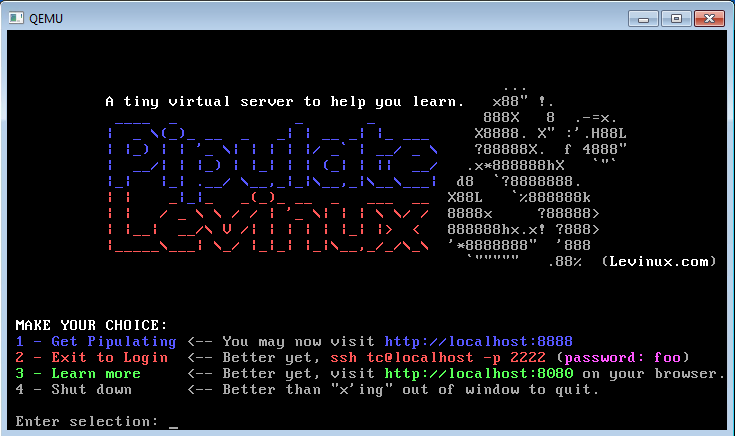
\includegraphics[width=0.75\textwidth]{images/levinux_welcome.png}
\caption{Levinux Welcome Screen}
\label{fig:levinux-welcome}
\end{figure}

\paragraph{} If you hit option 2 then you will immediately be able to log in to Levinux using the following credentials:

\begin{framed}
    \textbf{Username:} tc\blank{2cm} \textbf{Password:} foo
\end{framed}

\paragraph{} You should now see something like the following figure:

\begin{figure}[H]
\centering
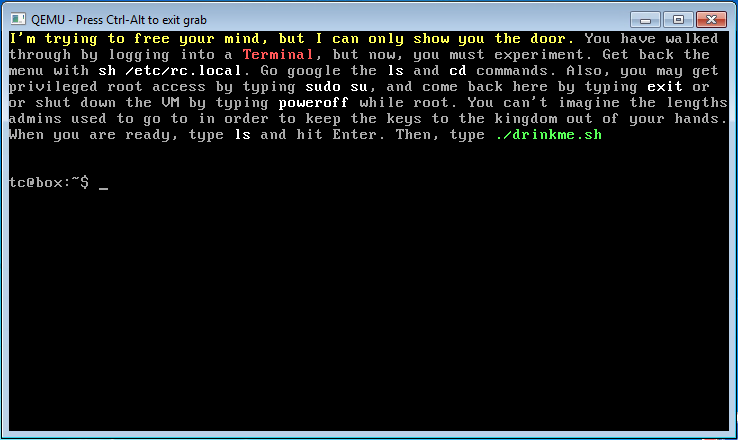
\includegraphics[width=0.75\textwidth]{images/levinux_loggedin.png}
\caption{The first screen after logging into Levinux}
\label{fig:levinux-logged-in}
\end{figure}

\paragraph{} At this point, Levinux is a minimal Linux system which has a basic set of tools but doesn't yet include any of the web development software or libraries that we will be using in this module. At this point you therefore have the option of jumping ahead to section \ref{linux} to learn a little more basic Linux, otherwise you could look at the SSH section which explains how to log in to Levinux multiple times using a tool called Secure Shell (SSH). If instead you want to get stuck in to getting your learning environment set up then you should proceed with the following steps which will install the following software:
\begin{enumerate}
\item Vim: A command-line based text editor
\item Python: A powerful programming language
\item Python-Flask: A Python library that makes it simple to build server-side web-applications
\item Various other supplementary libraries and tools that will help us to build some excellent web apps
\end{enumerate}

\paragraph{} These tools are not installed in Levinux by default because it keeps the size of the download smaller. NB. You can also install many other software packages from the Tiny Core Linux archive or from source code because this is, after all, a full Linux operating system installation. To install our extra software we do the following:

\subsection{Installing Vim}

\paragraph{} Log into Levinux if you haven't already done so then enter the following command at the prompt:
\begin{lstlisting}[style=DOS]
    tc@box:~$ ./drinkme.sh
\end{lstlisting}
\paragraph{} ./drinkme.sh runs a script that installs Vim. You will be prompted to confirm that this is what you want to do so enter `2' when asked(this might take a little while to completeas the software is being downloaded and installed into your virtual harddrive). Once the script is computer your should get your prompt back so that you can type more commands. You can launch Vim by typing `vim' at the prompt as follows (but if you are going to do that then you should probably take a look at section \ref{vim} of the notes which covers basic use of Vim):

\begin{lstlisting}[style=DOS]
    tc@box:~$ vim
\end{lstlisting}

\subsection{Installing the Web Development Environment}
\label{installing_environment}
\paragraph{} Again, if you are not logged in to Levinux then do so then enter the following command at the prompt: 

\begin{lstlisting}[style=DOS]
    tc@box:~$ sh ./Pipulate.sh 
\end{lstlisting}
\paragraph{} Again, just as for Vim, this runs a script called Pipulate.sh which installs Python, Python-Flask, a bunch of libraries, and Git. 

\paragraph{} These scripts basically sets up our development environment enabling us to edit, run, and control our source code.

\subsection{Shutting Down Levinux}
\paragraph{} The last thing we need to know about is how to safely shutdown our Levinux installation. Whilst logged in we can use the following command:
\begin{lstlisting}[style=DOS]
    tc@box:~$ sudo poweroff
\end{lstlisting}
\paragraph{} Which will cause Levinux to shutdown safely. If you are on the screen shown in figure \ref{fig:levinux-welcome} then you can just hit `4' then press $<$enter$>$. Remember, Levinux is a full computer system, even if it is running within another host system. Just as you wouldn't just hit the power button on your computer to turn it off, or at least you shouldn't, if you do that then stop it now. Instead, you should always follow the correct shut-down procedure for an operating system which gives it an opportunity to tidy itself up and clear up resources that are used. Doing anything else risks corrupting your installation so that it won't work correctly anymore and this is just as true for Levinux as it is for any other operating system.



\section{SSH}
\label{ssh}
\paragraph{} SSH which stands for `Secure Shell' is a tool for logging in to remote servers. We can use SSH to access Levinux as this provides us with an easy way to log in multiple times, e.g. have multiple shells (command lines) open and logged in to Levinux. The advantage of having multiple shells is that we can edit and save a program in one shell and run the program and monitor output in another shell. As you can imagine, this is very useful when we are developing new web apps on our Levinux server.

\begin{framed}
\textbf{IMPORTANT TIP} Once Levinux has booted, don't log directly into it. Instead, minimise the Levinux window and always log in using SSH, e.g. PuTTY, instead. This has many advantages but the main one is that you get a scrolling window so that you can see earlier commands or any output bigger than a single window of text. Additionally, PuTTy handles different keyboard layouts much better than Levinux so if you are using a French or German (or other) keyboard then this is the solution you need to get the keys you press to match the output on screen.
\end{framed}

\paragraph{} If you are on Linux or OS X then you will already have a version of SSH installed and all you need to do is open a terminal and type the following:

\begin{lstlisting}[style=DOS]
    $ ssh tc@localhost -p 2222
\end{lstlisting}

\paragraph{} then enter the password `foo' when prompted.

\paragraph{} However if you are on Windows then your will need to download an SSH client. The most popular client for Windows is called PuTTY\footnote{\url{http://the.earth.li/~sgtatham/putty/latest/x86/putty.exe}}. Download it, put it somewhere safe where you can access it then double click it to run. There is no need to install PuTTY as it is very portable. When PuTTY runs you will be presented with the following screen:

\begin{figure}[H]
\centering
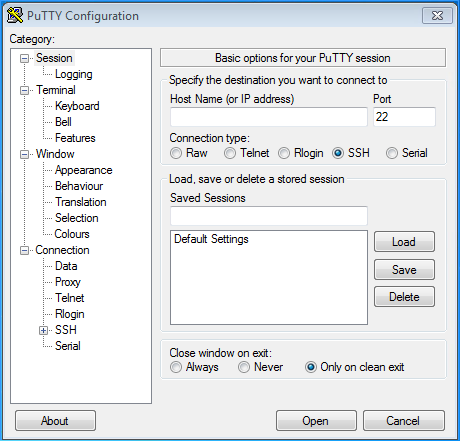
\includegraphics[width=0.5\textwidth]{images/putty_empty.png}
\caption{The PuTTY Window after you load it}
\label{fig:putty-empty}
\end{figure}

\paragraph{} You need to enter some connection details into this window as follows:

\begin{figure}[H]
\centering
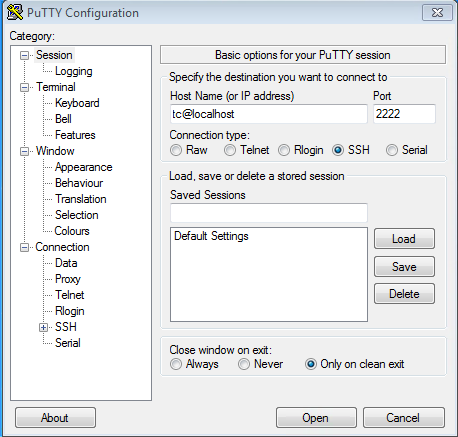
\includegraphics[width=0.5\textwidth]{images/putty_complete.png}
\caption{The PuTTY Window with completed connection details}
\label{fig:putty-complete}
\end{figure}

\paragraph{} You might be presented with the following window:

\begin{figure}[H]
\centering
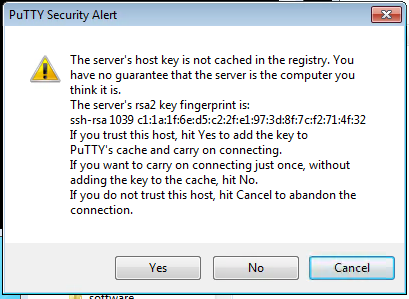
\includegraphics[width=0.5\textwidth]{images/putty_alert.png}
\caption{The PuTTY alert Window}
\label{fig:putty-alert}
\end{figure}

\paragraph{} If so, you can just click the `Yes' button. If all goes well you should now be presented with a login window for Levinux and all you have to do is type in the password (remember the password is `foo') and you should get a command line shell on your Levinux server.

\begin{figure}[H]
\centering
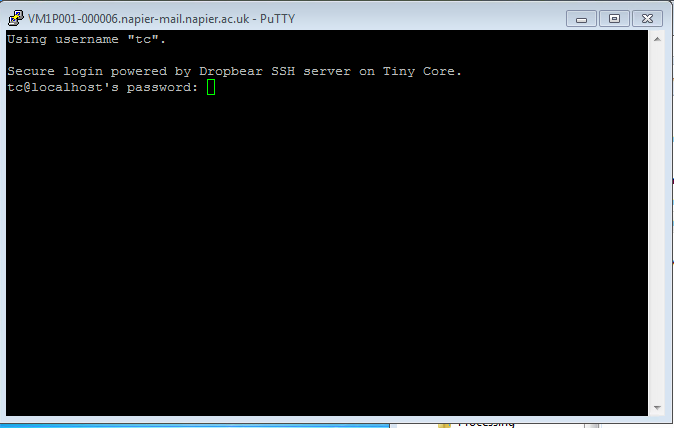
\includegraphics[width=0.75\textwidth]{images/putty_login.png}
\caption{The PuTTY login Window}
\label{fig:putty-login}
\end{figure}

\paragraph{} Remember, you can repeat this process with PuTTY as many times as required to get yourself enough shells into the Levinux server to make things easier to work with\footnote{This is not the best way to work with multiple shells. Another, more powerful way is to use a shell multiplexer, my favourite is one called Screen (\url{https://www.gnu.org/software/screen/}) but that is yet another tool to learn, and another set of commands, so lets try to keep things \emph{reasonably} simple}.

\begin{framed}
\textbf{IMPORTANT TIP} I usually use SSH to log into my Levinux installation at least twice. This gives me a window to edit text in and a window to test my code in. Often I will also have a third window open which I use for command line interaction, Git commits, and testing API calls using cURL, but two is the minimum for a nice development setup - Remember, this is your development environment so you might as well take some time to set it up nicely and so that you can work more productively.
\end{framed}


\section{Basic Linux Usage}
\label{linux}

\paragraph{} When we first log in to Linux we will see a prompt, a place where we can type commands. It looks something like this:

\begin{lstlisting}[style=DOS]
    tc@box:~$ 
\end{lstlisting}
\paragraph{} This simply means that user `tc' (short for tinycore, the default user that you logged in as) is logged into the machine called `box'. The `:' is merely a separate between the user@machine part of the prompt and the next part `{\raise.17ex\hbox{$\scriptstyle\sim$}}' which is your current location in the filesystem. The tilde or `{\raise.17ex\hbox{$\scriptstyle\sim$}}' symbol is used on Linux machines to mean your home directory.

\paragraph{} Linux has a file system, a way for all of the files that make up the running system to be organised hierarchically, just like Windows. However, on Linux the file system is organised a little differently. Instead of starting at `C:' the Linux file systems starts with `/' which is also known as the ``root'' of the filesystem. The word root is used because the Linux filesystem is shaped like a tree. All of the resources that you can access, such as your own files, are located at some level somewhere within the tree. An advantage of the Linux approach is that, when you add extra hard-drives, or mount network resources, instead of extra drive letters, all of your resources get mounted within the tree, e.g. /Volumes/Web might be the path to a remove web server and /media/cdrom might be the path to your CD-Rom drive. But other than that, from a basic user-oriented perspective, both Windows and Linux file systems are a hierarchical collection of files and directories in which any given directory might contain zero or more files or child directories.

\paragraph{} When you log in you will be located in your own directory, called your ``home'' directory which is located in the filesystem tree at 

\begin{lstlisting}[style=DOS]
    /home/tc
\end{lstlisting}
\paragraph{} You can see where you are in the filesystem by typing

\begin{lstlisting}[style=DOS]
    $ pwd
\end{lstlisting}
\paragraph{} which is short for print working directory or tell me where I am. You can type this anywhere you have a prompt. Also, no matter where you navigate to within the file system you can always return to your home directory by typing:

\begin{lstlisting}[style=DOS]
    $ cd
\end{lstlisting}

\paragraph{} You can navigate around the file system using the cd command which is short for `change directory'\footnote{You'll notice that many Linux commands are shortened versions of longer words. This is partly designed to reduce the amount of typing that you do. It may seem silly now but when you are changing directory hundreds of times a day it is much nicer to type cd than change-directory each time.}. The default version, without an argument takes you home, as we said before, but if you supply an argument then you can change the current directory. Let's try that now by changing to the root of the filesystem:

\begin{lstlisting}[style=DOS]
    $ cd /
\end{lstlisting}
\paragraph{} If you now use pwd you should see that the output is different to what it was before. You are no longer in your home directory but are in the root directory instead. Now ues the cd command without an argument to go home and use pwd to see where you are again. You can also step up through the directory hierarchy by using the `..' argument:

\begin{lstlisting}[style=DOS]
    $ cd ..
\end{lstlisting}
\paragraph{} `..' is an \emph{alias}, a label that has a default meaning, which in this case means ``move into the parent directory''. Explore the filesystem for a while using the cd, cd /, cd .., and pwd commands.

\paragraph{} There is a limit to what we can do with just these commands because we can only move into our home directory, or else navigate up through the tree to the file system root directory. We need a couple more commands to let us see what is inside a directory and to move into a new directory. For this we use the `ls' command which is short for list or list contents to see what files or child directories are in our current directory, and the cd command but with the name of a child directory as the argument. So, we can use `ls' as follows:

\begin{lstlisting}[style=DOS]
    $ ls
\end{lstlisting}

to list the files in the current directory. If you try this now you will see that your home directory contains a few default files and folders
e.g.

\begin{lstlisting}[style=DOS]
    tc@box:~$ ls
    Pipulate.sh  Recipe.sh    drinkme.sh   htdocs/
\end{lstlisting}

\paragraph{} Now we can create new files in our home directory quite easily using touch, e.g.

\begin{lstlisting}[style=DOS]
    $ touch testfile.txt
\end{lstlisting}

\paragraph{} which should give us something like this:

\begin{lstlisting}[style=DOS]
    tc@box:~$ ls
    Pipulate.sh   Recipe.sh     drinkme.sh    htdocs/       testfile.txt
\end{lstlisting}

\paragraph{} We can also create new directories using the `mkdir' which means make directory
\begin{lstlisting}[style=DOS]
    $ mkdir testdirectory
\end{lstlisting}

\paragraph{} which results in

\begin{lstlisting}[style=DOS]
    tc@box:~$ ls
    Pipulate.sh    drinkme.sh     testdirectory/
    Recipe.sh      htdocs/        testfile.txt
\end{lstlisting}
\paragraph{} We can also move files around using the `cp' and `mv' commands which are short for copy and move respectively. Let's see them in action; first we will make a copy of testfile.txt then move the copy into the testdirectory:
\begin{lstlisting}[style=DOS]
    tc@box:~$ cp testfile.txt testfile2.txt
    tc@box:~$ ls
    Pipulate.sh    drinkme.sh     testdirectory/ testfile2.txt
    Recipe.sh      htdocs/        testfile.txt
    tc@box:~$ mv testfile2.txt testdirectory/
    tc@box:~$ ls
    Pipulate.sh    drinkme.sh     testdirectory/
    Recipe.sh      htdocs/        testfile.txt
    tc@box:~$ ls testdirectory/
    testfile2.txt
\end{lstlisting}

\paragraph{} Notice that in this example we passed an argument, the name of a directory `testdirectory' to the ls command and this caused the contents of testdirectory to be listed instead of the current directory. We can do that with any directory that we have access to.

\paragraph{} Finally we might want to delete files to keep things tidy. We can use the `rm' command to remove files, e.g.
\begin{lstlisting}[style=DOS]
    tc@box:~$ rm testfile.txt 
    rm: remove 'testfile.txt'? y
    tc@box:~$ ls
    Pipulate.sh    Recipe.sh      drinkme.sh     htdocs/        testdirectory/
\end{lstlisting}
\paragraph{} We can use also use rm to remove directories, however, by default we get this behaviour:
\begin{lstlisting}[style=DOS]
    tc@box:~$ rm testdirectory/
    rm: 'testdirectory' is a directory
\end{lstlisting}
\paragraph{} What we need to do instead is to supply some options to the rm command. We need rm to act recursively, that means move into the specified directory and delete its contents and we also need to force rm not to stop and ask us for each file whether it should be deleted. We there fore need to use rm as follows:
\begin{lstlisting}[style=DOS]
    tc@box:~$ ls
    Pipulate.sh    Recipe.sh      drinkme.sh     htdocs/        testdirectory/
    tc@box:~$ rm -rf testdirectory/
    tc@box:~$ ls
    Pipulate.sh  Recipe.sh    drinkme.sh   htdocs/
\end{lstlisting}
\paragraph{} Of all the commands we have met so far, rm is the only one that can do any real damage. rm -rf could conceivably delete all of your files and directories if the command is executed in the wrong place. As a rule it is probably worth only making changes within your home directory, e.g. /home/tc, whilst working on exercises in this module, that way you are less likely to destroy your Levinux install accidentally and have to start again. However because it is easy to set up and run a new Levinux instance you can afford to experiment because if you destroy your Levniux instance you can always start again. You should however, especially once you start writing code in Levinux, keep backups of anything that you will need to use again such as the code for your courseworks.

\paragraph{} There are many, many more commands than just these. In fact you can do much more with the command line than you can with graphical tools. However, this should be enough for you to get started and is enough for you to be able to create and delete files and directories, to navigate the file system hierarchy, to list the contents of directories, and to view the contents of files. 

\paragraph{} To do more exploration of Linux, you can of course experiment with Levinux. Another good place to start is the Linux Zoo site\footnote{\url{http://www.linuxzoo.net}} which offere online virtual machines, more information, and a number of tutorials. Particularly the Linux Zoo ``essential Linux'' pages\footnote{\url{http://linuxzoo.net/page/intro.html}} which explain in more depth some of the tools that we have already covered plus many many more.








\section{Vim}
\label{vim}
\paragraph{} Vim is a command-line based text editor. It is based on an earlier editor called Vi (Vim is VI improved, hence Vim, which is a little easier to use). You might ask why we don't just use a GUI text editor like Notepad, or the editor in Visual Studio. The main reason is because we are talking about advanced web technologies, and dealing with them often involves accessing remote servers. Furthermore, the majority of servers do not have a graphical interface and only have installed the most minimal and robust set of tools. The one editor that you are almost guaranteed to find on any Unix or Linux server is Vi and by learning Vim you are well placed to handle Vi. As a result it makes sense for us to become familar with it. Many of us actually find that the shortcuts and powerful control that Vim offers us mean that we just concentrate on learning one editor very well and only use that editor rather than moving to a different editor each time we need to write a different type of document or program in a different language.

\paragraph{} What makes Vim different from many of the editors that you will be familar with, like Notepad, is that there is no role for the mouse, no buttons to click at all, only keyboard shortcuts, so we shall learn just enough of those in this module to be able to edit basic documents\footnote{However there are hundreds of Vim commands and a really clever things is that most of the commands can be chained together so that you can automate many editing tasks.}. A second very important aspect of Vim is that it is a \emph{modal} editor. When you use Vim you use it in different modes, when you are typing content into a file then you are in edit mode, and when you are entering commands you are in command mode. When Vim starts it is in command mode and anything you type will be interpreted as a command for Vim to perform. You switch into edit mode by typing `i' (for insert) and you can return to command mode at any time merely be hitting the escape key.

\begin{framed}
\textbf{IMPORTANT} If you are ever unsure what mode you are in the you can just hit escape a couple of times to ensure you are in edit mode. From here you can just type `i' again to enter the edit mode.
\end{framed}

\paragraph{} Start Vim by typing Vim at the prompt:
\begin{lstlisting}[style=DOS]
    tc@box:~$ vim
\end{lstlisting}
\paragraph{} and you will see something similar to the following:

\begin{figure}[H]
\centering
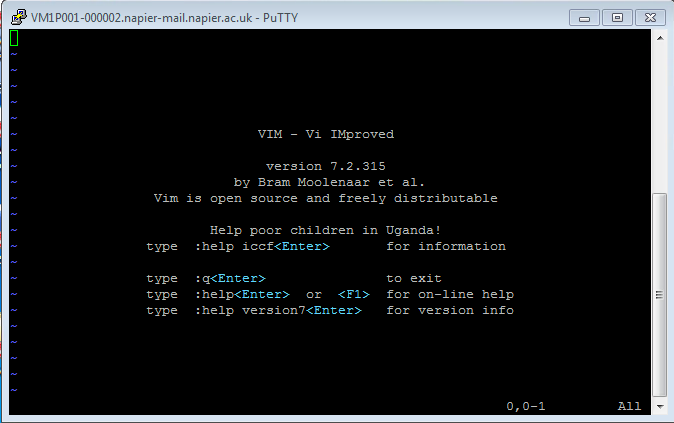
\includegraphics[width=0.75\textwidth]{images/vim_first.png}
\caption{The default Vim Editor window}
\label{fig:vim-first}
\end{figure}

\paragraph{} Let's do the easiest thing first. Let's quit Vim. To do this we enter the command mode by hitting escape then enter `:q' (where is q is short for quit) and hit enter, e.g.

\begin{lstlisting}[style=DOS]
    <ESC>:q<ENTER>
\end{lstlisting}
\paragraph{} Your Vim window should look something like this when the command is entered (but before you press enter):

\begin{figure}[H]
\centering
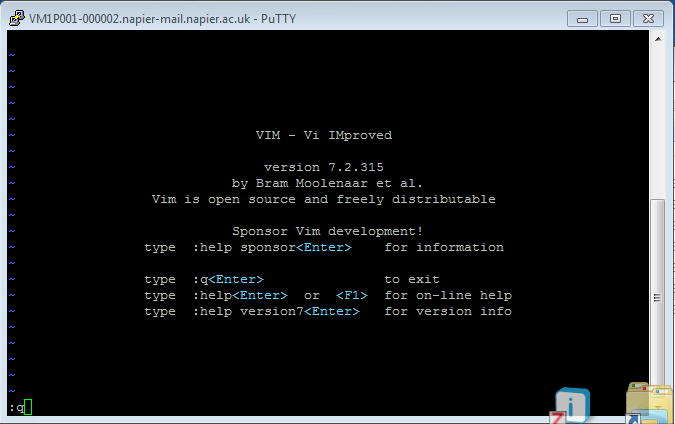
\includegraphics[width=0.75\textwidth]{images/vim_quit.png}
\caption{The Vim Editor with `:q' command entered}
\label{fig:vim-quit}
\end{figure}

\paragraph{} Once you hit enter you will be dumped back to the Linux prompt. Two other useful commands to be aware of for quitting are as follows:

\begin{itemize}
\item To quit and discard any changes, i.e. if you have already made changes to a document that you don't want to save:\\
\begin{lstlisting}[style=DOS]
    <ESC>:q!<ENTER>
\end{lstlisting}
\item To quit and save changes, we use :wq for (w)rite and (q)uit:
    \begin{lstlisting}[style=DOS]
    <ESC>:wq<ENTER>
\end{lstlisting}
\end{itemize}

\paragraph{} Let's start Vim again and actually edit some text. This time when Vim starts you need to press `i' for (i)nsert to enter the edit mode. You can now type away to your hearts content. When you are ready to save the file you can enter the command mode and type :w for (w)rite. If the file doesn't have a filename you will get a message to that effect so, with a new file that isn't yet saved you can us :w filenname.txt (where filename.txt is the name of the file that you want to create). This file will then be created in whichever directory you were in when you started Vim.

\paragraph{} There is \textbf{A LOT} to learn in Vim. The easiest way to do that is to just use it. There are many online resources that teach you how to use Vim but two of my favourites are:
\begin{enumerate}
\item The Open Vim Tutorial: \url{http://www.openvim.com/}
\item Vim Adventures: \url{http://vim-adventures.com/}
\end{enumerate}

There is also a cribsheet of useful commands in section \ref{cribsheet_vim}.

\section{Git}
\label{git}
\paragraph{} Git is a source control system that enables you to keep track of your source code, its history and any changes you make. Git can be used to track any file but is most efficient and best suited when used only with textual files. Because Git is a \emph{distributed} source control system it works very well to enable groups of people to work on the same source code as well as supporting experimenting with your code, trying out lots of different ideas in separate \emph{branches} (which are a bit like a copy of your code but with tools to help manage that copy and support re-integrating it with your main source tree if you want to), and being able to roll back to an earlier version if you decide you have take a wrong turn.

\paragraph{} Whilst you might have seen Git before, perhaps as a plugin to an IDE or as a standalone GUI app, Git is primarily a command line application, so we shall use it to get our source code in and out of Levinux.

\begin{framed}
\textbf{IMPORTANT} We shall use Git to support the hand-in of courseworks in this module so you should get familiar with it as soon as possible. A good place to start is by dipping into the Git SCM book\footnote{\url{http://git-scm.com/book/en/v2/Getting-Started-About-Version-Control}}.

\paragraph{} There are also numerous interactive tutorials and resources to help you get started with Git:
\begin{enumerate}
\item Github's Learn Git 15 minute tutorial: \url{https://try.github.io/levels/1/challenges/1}
\item Learn Git Branching \url{http://pcottle.github.io/learnGitBranching/}
\item Git Immersion \url{http://gitimmersion.com/lab_01.html}
\end{enumerate}

\paragraph{} You should also create either a Github account\footnote{\url{https://github.com/}} or a Bitbucket account\footnote{\url{https://bitbucket.org}} (or both if you like) then create a repository within your new account called `set09103'. You will push all of your code throughout the module into this repository and at hand in time I will pull a copy for marking. The advantage of this appraoch is that at any point, if you need help with your code, then we have a copy that I can see remotely. However this only works if you keep adding your code to your repository. That means whenever you make changes you need to (1) add them, (2) commit them with an explanatory message,  and (3) push the changes from your local repository to the shared one on Github or Bitbucket.

\end{framed}

\paragraph{} Once you have gone through the steps in section \ref{installing_environment} you will already have Git installed in Levinux. In order to use it we have to do a couple of things. Log into Levinux then do the following (obviously replace my email address and name with your own):
\begin{lstlisting}[style=DOS]
    $ git config --global user.email "s.wells@napier.ac.uk"
    $ git config --global user.name "Simon Wells"
\end{lstlisting}

\paragraph{} It is easiest to create a new repository through the interface on Github or Btbucket then use the repository cloning address to make a local copy as this sets up all the addresses automatically for pushing and pulling code. Once a repository is set up and you have cloning address you can do something similar to the following (where \url{https://siwells@github.com/siwells/sandpit.git} is the name of one of my repositories on github, your's will obviously be different):

\begin{lstlisting}[style=DOS]
    $ git clone https://siwells@github.com/siwells/sandpit.git
\end{lstlisting}

\paragraph{} We can then make changes within the new local clone of, in this case the `sandpit' repository, then add, commit, and push as follows (again the details of adding and committing depend upon the exact files that you have altered. In this case we'll assume that a file test.txt has been edited):

\begin{lstlisting}[style=DOS]
    $ git add .
    $ git commit -m "Added introductory example"
    $ git push
\end{lstlisting}

\paragraph{} Again, as for Linux and Vim, there are many options and powerful features that you can learn to use with Git, however we shall try to keep things as simple as possible for now.

\begin{framed}
\textbf{ADVANCED} If you are comfortable with using Git and SSH then you might want to try setting up SSH keys so that you don't have to use a password each time you push code into your remote repository.
\end{framed}

\section{Wrapping Up}
\label{chapter_01_wrap-up}
\paragraph{} Obviously this has only been the most basic of introductions to web development using a Linux server. There is much much more that you could learn about any one of the tools that we have introduced and it is well worth your time to explore additional resources and reading for each of them. It is very likely that you will experience some or even all of these technologies, in some form, at some point of your career and putting in some extra effort now will mean that you are much more capable later.

%%%%%%%%%%%%%%%%%
%%%%%%%%%%%%%%%%%
% CHAPTER 2
%%%%%%%%%%%%%%%%%
%%%%%%%%%%%%%%%%%

\chapter{Learning Environment Part \#2}
\label{lab2}
\paragraph{} After last weeks extravaganza of new tools, we will only introduce two new tools this week, the Python language and a Python Library for developing web applications called Flask. By the end of this weeks practical work you should be able to build a simple `Hello Napier' web app using Python and Python-Flask which is hosted on and runs within our simple Levinux Virtual Linux environment and whose source code is pushed to our personal Github (or Bitbucket) repositories. 

\begin{framed}
\textbf{VERY IMPORTANT} The work this week builds directly on last week so if you haven't finished working through chapter \ref{lab1} then it is best to do that first or you will probably get horribly stuck.
\end{framed}

\section{Python}
\label{python}
\paragraph{} Python\footnote{\url{https://www.python.org/}} is a very useful programming language and much of its popularity stems from the fact that it is easy to get a lot done with having to write too much code. We already have Python installed in Levinux and ready to use. We can run Python by typing its name in the terminal, e.g.

\begin{lstlisting}[style=DOS]
tc@box:~$ python
Python 2.7.10 (default, May 25 2015, 09:55:35) 
[GCC 4.9.1] on linux2
Type "help", "copyright", "credits" or "license" for more information.
>>> 
\end{lstlisting}
\paragraph{} This starts the Python Read-Evaluate-Print-Loop or REPL in which we can type Python commands and get immediate output. To exit the REPL we type `quit()' which will return us to the Linux shell, e.g.

\begin{lstlisting}[style=DOS]
tc@box:~$ python
Python 2.7.10 (default, May 25 2015, 09:55:35) 
[GCC 4.9.1] on linux2
Type "help", "copyright", "credits" or "license" for more information.
>>> quit()
tc@box:~$ 
\end{lstlisting}

\paragraph{} Here is the traditional `Hello Napier' program in Python (try it out for yourself):

\begin{lstlisting}[style=DOS]
tc@box:~$ python
Python 2.7.10 (default, May 25 2015, 09:55:35) 
[GCC 4.9.1] on linux2
Type "help", "copyright", "credits" or "license" for more information.
>>> print "Hello Napier"
Hello Napier
>>> quit()
tc@box:~$
\end{lstlisting}

\paragraph{} The REPL is very useful for trying out bits of Python as you are learning and also for interactively developing code and analysing data. There are super-charged REPLs and related tools such as iPython\footnote{\url{http://ipython.org/}} and iPython notebooks\footnote{\url{http://ipython.org/notebook.html}} which are used in data science and data analysis. However, once we are comfortable with the Python syntax, we will mostly want to run Python scripts, so let's do that.

\paragraph{} Create a new file called first.py, open it in Vim then edit it as follows:

\begin{lstlisting}
print "Hello Napier"
\end{lstlisting}

\paragraph{} Save and close first.py then execute the following command in the shell:

\begin{lstlisting}[style=DOS]
    tc@box:~/src$ python first.py 
    Hello Napier
    tc@box:~/src$
\end{lstlisting}

\paragraph{} Congratulations. Another first. You just ran your very first Python script. All we will really do from now on in the remainder of this module is build on top of this basic script in order to build our own web-apps. However, we shall have some help along the way from some really excellent libraries so don't worry, we shan't build everything from scratch.

\paragraph{} Now the best thing to do is to learn some Python syntax by exploring som of the excellent online `learn Python' tutorials that are available. Some of them are interactive, so you can type directly into the web-site and get results. Others just give you exercises to do yourself and you can do those exercises in Python on our Levinux platform. Here are a few, in order of usefulness according to me, but many more are just a Google search away:

\begin{enumerate}
\item Learn Python the hard way: \url{http://learnpythonthehardway.org/book/}
\item The Python Practice Book: \url{http://anandology.com/python-practice-book/index.html}
\item A Byte of Python: \url{http://www.swaroopch.com/notes/python/}
\item Code Combat: \url{https://codecombat.com/}
\item Python for you and me: \url{http://pymbook.readthedocs.org/en/latest/}
\item The Hitchhiker's Guide to Python: \url{http://docs.python-guide.org/en/latest/#the-hitchhiker-s-guide-to-python}
\item Hands-On Python Tutorial: \url{http://anh.cs.luc.edu/python/hands-on/3.1/handsonHtml/index.html}
\item The Python Challenge: \url{http://www.pythonchallenge.com/} - Some quite touch challenges that you can solve using Python (NB. Assumes you already know what you are doing)
\item Python Tutor: \url{http://www.pythontutor.com/} - Helps visualise the execution of Python code. Again, assumes that you have some prior knowledge of Python syntax.
\end{enumerate}

\paragraph{} The links towards the top of the list are aimed at those completely new to the Python language whereas those further down the list will help those who have some Python knowledge already. Another good way to practice a new language or to improve your existing abilities, not just in Python, but in any language, is to try to solve a set of problems using the language. I often use Project Euler when starting out with a new language but there are also many others:

\begin{enumerate}
\item Project Euler: \url{https://projecteuler.net/}
\item Stack Exchange Code Golf: \url{http://codegolf.stackexchange.com/}
\item Code kata: \url{http://codekata.com/}
\item Reddit Daily Programmer: \url{https://www.reddit.com/r/dailyprogrammer}
\item Programming Praxis: \url{http://programmingpraxis.com/}
\item Rosetta Code: \url{http://rosettacode.org/wiki/Main_Page}
\item International Collegiate Programming Contest Problems Index: \url{http://acm.hit.edu.cn/judge/ProblemIndex.php}
\item Algorithmist: \url{http://www.algorithmist.com/index.php/Main_Page}
\end{enumerate}

\paragraph{} It is also worth creating a git repository of any code that you create when learning a new language because if you take a break from that language to do something else, you will have somethings to remind you of where you were up to before. It is also a neat way to share your solutions with others. If you exhaust all that lot then another great practice approach is to try to implement your own versions of basic (and advanced) algorithms and data structures. For example, if you really want to challenge yourself, and your knowledge of a programming language, read about and implement probabilistic datastructures like Bloom Filters which I find quite interesting, or Fountain Codes which are used in tools like Bittorrent.

\section{Python-Flask}
\label{python-flask}
\paragraph{} Python-Flask, or just Flask\footnote{\url{http://flask.pocoo.org/}}, is a Python based microframework for developing websites in Python. If you have run the drinkme.sh and Pipulate.sh scripts from Chapter \ref{lab1} then Flask will already be installed and ready to run. We shall leave all of the nitty gritty of installing and administrating software on a Linux server as an exercise that is outside of the remit of this module and just focus on using the tools now that we have them.

\paragraph{} Flask includes a lot of useful tools; a development server and debugging tools so that we can run our flask apps during development without needing to run a separate external server like Apache\footnote{\url{http://www.apache.org/}} or NGinX\footnote{\url{https://www.nginx.com/resources/wiki/}}. Obviously if we were deploying our apps in the real world then we would host our web-apps differently. We would use a secure Linux install on a server with access to the external world and would use a good HTTP server, like NGinX, and a WSGI-compliant app-server, like uWSGI\footnote{\url{https://uwsgi-docs.readthedocs.org/en/latest/}}. We might even use a load balancer like Haproxy\footnote{\url{http://www.haproxy.org/}} to enable us to scale our operations. We will look at all of these aspects later in the module but for now we shall concentrate on the development server and a simplified development environment. Flask also has integrated unit-testing support, RESTful request dispatching, templating, to help generate HTML pages, using the Jinja2 tool.

\paragraph{} Flask supports us in building web-apps that conform to the Python Web Server Gateway Interface (WSGI)\footnote{The WSGI standard is described in this Python Pep:\url{https://www.python.org/dev/peps/pep-0333/}. A PEP is a Python Enhancement Proposal and is the main way that the planned development of the Python language progresses.}. The goal of WSGI is to make it easy to develop and deploy Python web-app, regardless of the library that is used. So developers can find a library that they find useful, or helps them to tackled their development task, but the output of the process, the web-app has know features and capabilities which means that any server that supports the WSGI can run the web-app. This is similar to what happened with web-app development in Java, where the servlet API means that many tools can be used to build a Java web-app and many web-servers can then run the app.

\begin{framed}
\textbf{IMPORTANT} The version of Levinux that we have used from the \url{http://levinux.com/} site does not forward port 5000. This is the port that we will access in our browser to see our web-apps. We have two solutions, the first is to download a new version of Levinux (Napier Edition) from the SET09103 Moodle page and set up a fresh environment (you will have to run the pipulate and drinkme scripts again. The alternative, which might wreck your version of Levinux and mean you have to start again anyway is to edit two of the startup scripts within Levinux. To ensure that your installation stays completely portable there are scripts to edit. The first is here Pipulate.app/Contents/MacOS/qemu32.bat and you need to add the following line between the similar lines for higher and lower port numbers:
\begin{lstlisting}
    -redir tcp:5000::5000 ^
\end{lstlisting}
Similarly we need to edit the Pipulate.app/Contents/Resources/qemuonmac.sh file to add the following line:
\begin{lstlisting}
    -redir tcp:5000::5000 \
\end{lstlisting}
Ensure that both edits are exactly as shown. If you have done it wrong then worst case scenario is that your Levinux install won't start. The othe likely failure is that Levinux will start but the port won't forward properly.
\end{framed}

\section{Python Flask ``Hello Napier''}
\label{hello-napier}
\paragraph{} Here is our first Python Flask app:

\begin{lstlisting}
from flask import Flask
app = Flask(__name__)

@app.route("/")
def hello():
    return "Hello World!"

if __name__ == "__main__":
    app.run(host='0.0.0.0')
\end{lstlisting}

\begin{framed}
\textbf{IMPORTANT} Don't just copy and paste code from the PDF. This is for two very good reasons. The first is that Python is `white-space sensitive'. This means that Python uses whitespace as part of the layout of code, instead of using things like curly braces such as `\{' and `\}'. So if you get spaces, tabs, and other whitespace characters mixed up in your file, which can easily happen if you copy and paste, then it will affect the indentation of the file (although perhaps not in a way that you can tell visibly because whitespace can all look pretty much the same). The second very good reason is that typing in the code counts as `deliberate practise'. You are more likely to remember stuff if you do it multiple times and typing it in the first time counts as the first opportunity to practise.
\end{framed}

\paragraph{} Type in the `Hello Napier' code from above or get it from the module's Git repository. Save the code in a file called hello.py then run it by executing the following command in the same directory where hello.py is stored:

\begin{lstlisting}[style=DOS]
    $ python hello.py
\end{lstlisting}

\paragraph{} This command causes our web-app to be run using the Flask development server which is really useful and fast for debugging during development. If everything goes well then you should see output similar to the following in your terminal:

\begin{lstlisting}[style=DOS]
tc@box:~$ python src/hello.py 
 * Running on http://0.0.0.0:5000/ (Press CTRL+C to quit)
 * Restarting with stat
\end{lstlisting}

\paragraph{} Congratulations. You now have your first Python web-app running. You can visit the page generated by Flask in a web browser. Just start up a browser in your host OS, e.g. in Windows when running Levinux in the lab. Although the output from Flask in your terminal tell you which address (and port) your app is running at '0.0.0.0' doesn't appear to reliably resolve on Windows so it is best to navigate to \url{localhost:5000}:

\begin{figure}[H]
\centering
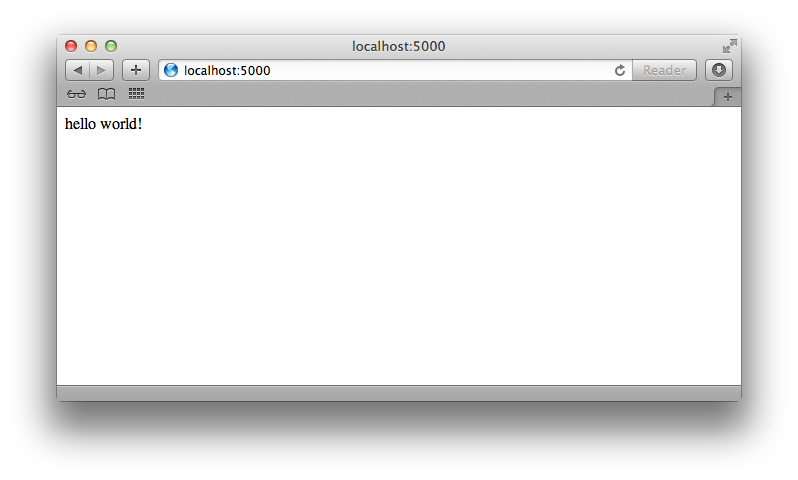
\includegraphics[width=0.8\textwidth]{images/flask-hello-napier.png}
\caption{Your first Python Flask web app.}
\label{fig:flask-hello-napier}
\end{figure}

\section{Wrapping Up}
\label{chapter_02_wrap-up}
\paragraph{} Right. Thats all the preliminaries in place for building web-apps in our learning environment. We can now run a small and lightweight, but otherwise similar to full Linux installs, virtualised server which will host our web-apps. We can log in to the server using SSH, navigate the Linux environment, and edit files using VIM. We can also take advantage of the installed Python language and Python-Flask web-app library to build our own web-apps.

\begin{framed}
\textbf{CHALLENGE} Create a Github or Bitbucket account. Bitbucket allows you to create an unlimited number of private repositories if you use your @napier address to register whereas Github restricts the number of private repos. That said, either site allows you to create as manay public repositories as you like. Create a remote repo in your Github or Bitbucket account called `set09103'. Run Levinux and log in then clone your set09103 repo. Create a new file in your repo called `hello.txt' and put the message ``Hello Simon'' in it then add, commit and push your changes to your remote repo. Once you have done this, check on either Github or Bitbucket to ensure that your text file is in the repo where you expect it to be then send an email to Simon containing the name of your account, which service, Github or Bitbucket, you are using, and the clone url for your set09103 repository. {\emph{If you use a private repository then you will have to add my account as a collaborator. On both Github and Bitbucket my account name is `siwells'}}. I will then pull everyone's repos to ensure that we are all at the same place in our learning. We will then use the set09103 repos as the place to store our coursework projects and for the hand-in. This just means that we have everything in place early before the hand-in deadline.
\end{framed}

\paragraph{} Over the next few chapters we will look at a whole host of things we can do with Flask. However you should also rest assured that all of the tools we are learning will prove useful to you at some point in your career and will help you to become the best developers that you can be.

%%%%%%%%%%%%%%%%%
%%%%%%%%%%%%%%%%%
% CHAPTER 03
%%%%%%%%%%%%%%%%%
%%%%%%%%%%%%%%%%%


\chapter{Python Flask: Debug Mode, Errors, Routing, \& Static Files}
\label{lab3}
\paragraph{} The last two weeks have got us to the point where we can build a simple `Hello Napier' web app using Python and Python-Flask hosted within our simple Levinux Virtual Linux environment and whose source code is pushed to our personal Github (or Bitbucket) repositories. We can now start to expand our web-app skills using Python-Flask. We'll start by looking at the debug mode which enables us to tell the Flask development server to do hot reloads of updated code whenever we save our edited python web-app file. This saves us lots of time as we begin to make lots of changes to our web-app. Additionally, we should expect to to see lots of errors. After all we are working with lots of new tools. So we shall look at Flask errors and how to deal with them. Then we will look at routing requests from web browsers to different URLs, basically how to build a tree of web addresses that each fire off a different Python function when the browser tries to access them. Finally we will look at serving up static files, like image files from the file system.

\begin{framed}
\textbf{VERY IMPORTANT} Chapters for this and subsequent weeks build directly on all of the skills learned in the first two chapter, particularly Levinux, Linux, SSH, and Vim from chapter \ref{lab1} and Python and Python Flask from \ref{lab2}.

\paragraph{} To some degree you can mix and match this and subsequent chapters and subsections to meet your needs, for example, the type of web app you want to build, but you should aim to cover all chapters by the end of the semester.
\end{framed}

\section{Flask Debug Mode}
\label{debug}
\paragraph{} Recall that our `Hello Napier' app looks like this:

\begin{lstlisting}
from flask import Flask
app = Flask(__name__)

@app.route("/")
def hello():
    return "Hello World!"

if __name__ == "__main__":
    app.run(host='0.0.0.0')
\end{lstlisting}

\paragraph{} When we run this Python flask app using the python command in the terminal, e.g.

\begin{lstlisting}[style=DOS]
tc@box:~$ python src/hello.py 
 * Running on http://0.0.0.0:5000/ (Press CTRL+C to quit)
 * Restarting with stat
\end{lstlisting}

\paragraph{} Python calls the run function of the app object and executes it. By default run() takes no arguments but we have used the \emph{host='0.0.0.0'} argument to tell flask to allow connections from outside of the local machine, this is what enables us to access the web-app from Windows as by default we would only be able to access the web-app from within Levinux. However both the app object and the run function have a number of other features that we can use. Whilst developing a new web-app one of the most important is the debug mode which we can run by adding debug=True to our call of the run function, e.g.

\begin{lstlisting}
    app.run(host='0.0.0.0', debug=True)
\end{lstlisting}

\paragraph{} Two important features of the debug mode are

\begin{enumerate}
\item Causing the development server to automatically restart each time we change our code, e.g. each time we save (\emph{:w $<$ENTER$>$}) our file after editing it in Vim.
\item Printing out debug information and a Python stack trace in the browser so that we can work out what went wrong.
\end{enumerate}

\paragraph{} If we try to access a route that causes a Python error then instead of this

\begin{figure}[H]
\centering

\includegraphics[width=0.9\textwidth]{images/flask-internal-server-error.png}
\caption{Flask internal server error}
\label{fig:flask-internal-server-error}
\end{figure}
 \paragraph{} We will get a Python stack trace displayed in the browser (and printed on the output in the terminal where you ran the web-app). Here is an example but remember that the stack trace will differ greatly depending upon the type of error and the details of what went wonge so this is merely indicative:

\begin{figure}[H]
\centering
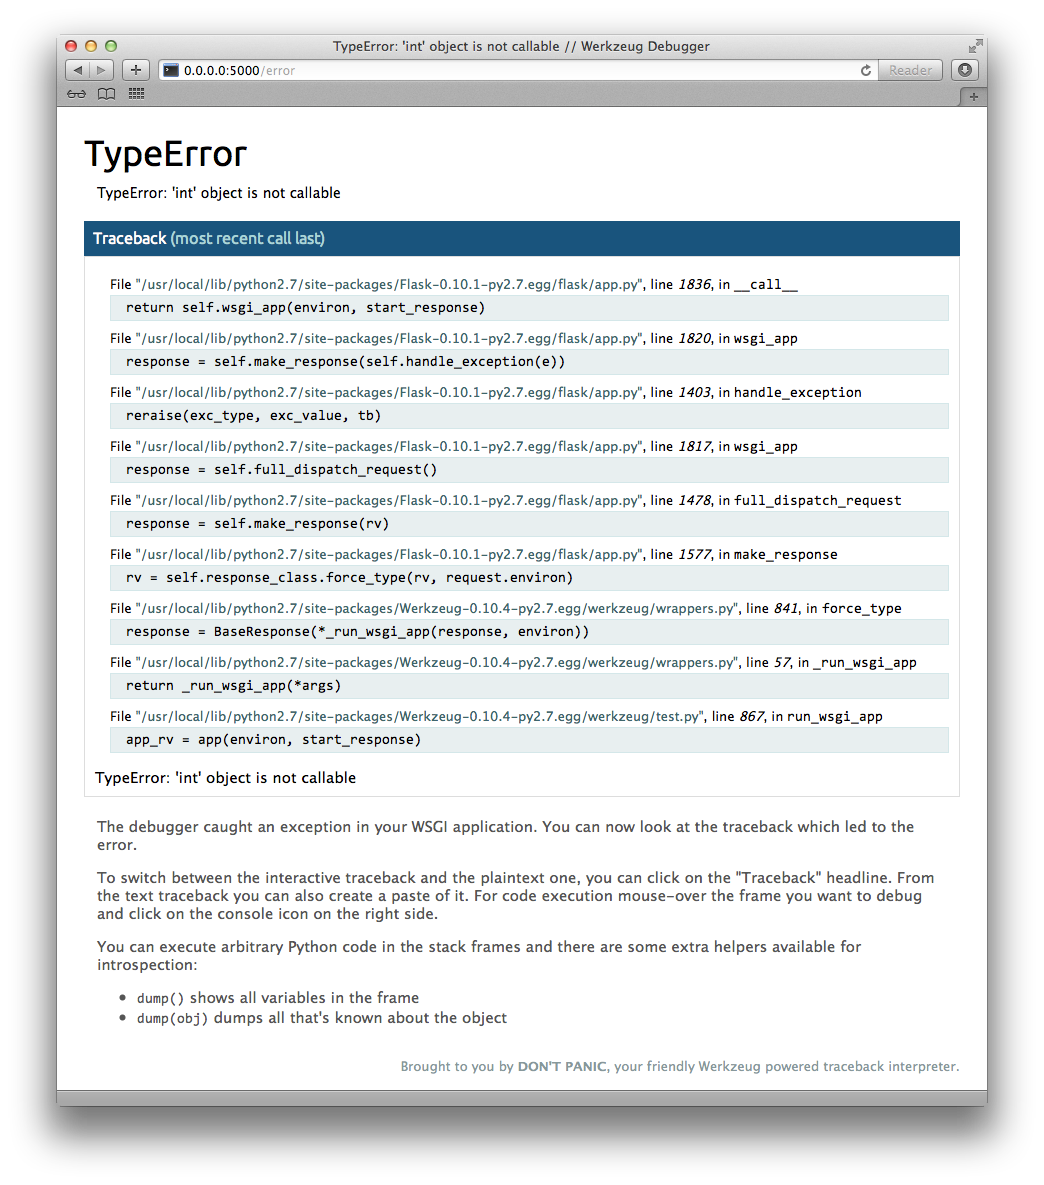
\includegraphics[width=0.9\textwidth]{images/flask-stack-trace.png}
\caption{An error stack trace example}
\label{fig:flask-stack-trace}
\end{figure}


\begin{framed}
\textbf{IMPORTANT} If you ever run your web-app on a publically accessible server then you must turn debug mode off as it presents a significant security risk and can allow the execution of arbitrary code.
\end{framed}

\section{Flask Routing}
\label{routing}
\paragraph{} Routing is what enables us to build sensible URLs and addresses for the pages of our web-app. You should consider the design of the address hierarchy for your web-app, the API, to be at least as important a consideration as the design of any content of your actual web-apps pages.

\paragraph{} In flask, web addresses or URLs are called routes. To add more routes to your web-app you use the app.route decorator. You just write a new Python function then add a decorator for each one to make the function into a route. For example, in the following web-app we have 3 routes:

\begin{lstlisting}
from flask import Flask, redirect, url_for, abort
app = Flask(__name__)

@app.route("/")
def root():
  return "The default, 'root' route"

@app.route("/hello/")
def hello():
  return "Hello Napier!!! :D"

@app.route("/goodbye/")
def goodbye():
  return "Goodbye cruel world :("

if __name__ == "__main__":
  app.run(host='0.0.0.0', debug=True)
\end{lstlisting}

\section{Flask Redirects \& Errors}
\label{errors}
\paragraph{} You can redirect a user from one URL endpoint to another quite easily by using the redirect() function, for example, if we were building an app that required a user to be logged and we detected that the user wasn't logged in then we could redirect the user to a login page instead of the page that they requested, e.g.

\begin{lstlisting}
from flask import Flask, redirect, url_for
app = Flask(__name__)

@app.route("/private")
def private():
  # Test for user logged in failed
  # so redirect to login URL
  return redirect(url_for('login'))

@app.route('/login')
def login():
  return "Now we would get username & password"

if __name__ == "__main__":
  app.run(host='0.0.0.0', debug=True)
\end{lstlisting}
\paragraph{} Note that this isn't an entire web-app, just the imports and indicative code for how a redirect could work. Obviously, to complete the scenario above we would also need code to check whether the request came from a logged in user and the login page would also need to accept and check any supplied credentials (but we will look at that type of functionality in subsequent chapters). 

\paragraph{} If we try to access a page that doesn't exist then we get a default error 404 Not Found status page like the following:

\begin{figure}[H]
\centering
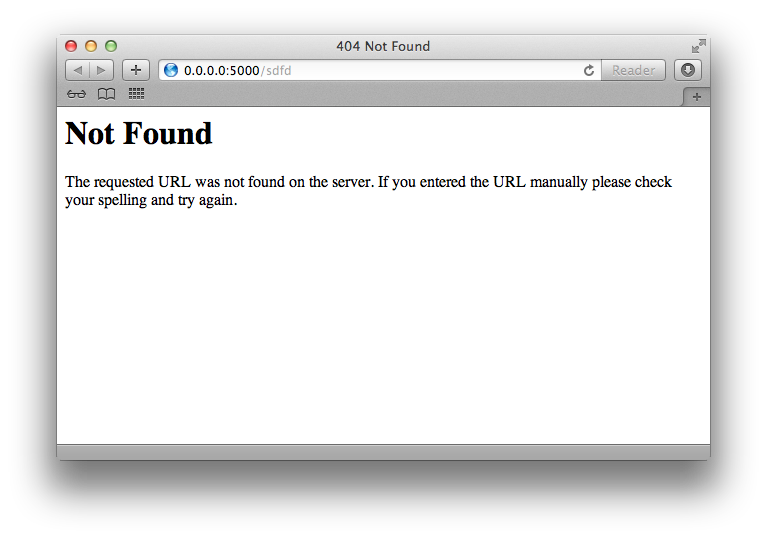
\includegraphics[width=0.9\textwidth]{images/flask-not-found.png}
\caption{The default 404 Not Found page}
\label{fig:flask-not-found}
\end{figure}

\paragraph{} However we can also provide our own error pages that better fit in with the design of our app or tell our user how to recover from the error. For example, you could provide a link to the root page or login page instead. Providing a custom HTTP error page is straightforward. Instead of the \emph{@app.route} decrator we use the \emph{app.errorhandler} decorator and pass it the code that we want to handle. We also add the code after the return message so that the code is returned to the browser.

\begin{lstlisting}
from flask import Flask
app = Flask(__name__)

@app.route("/")
def hello():
  return "Hello Napier"

@app.errorhandler(404)
def page_not_found(error):
  return "Couldn't find the page you requested.", 404

if __name__ == "__main__":
  app.run(host='0.0.0.0', debug=True)
\end{lstlisting}

\paragraph{} Now if we visit our web-app but use an address that doesn't exist (just make something up after the http://localhost:5000/ bit) we should see something like this:

\begin{figure}[H]
\centering
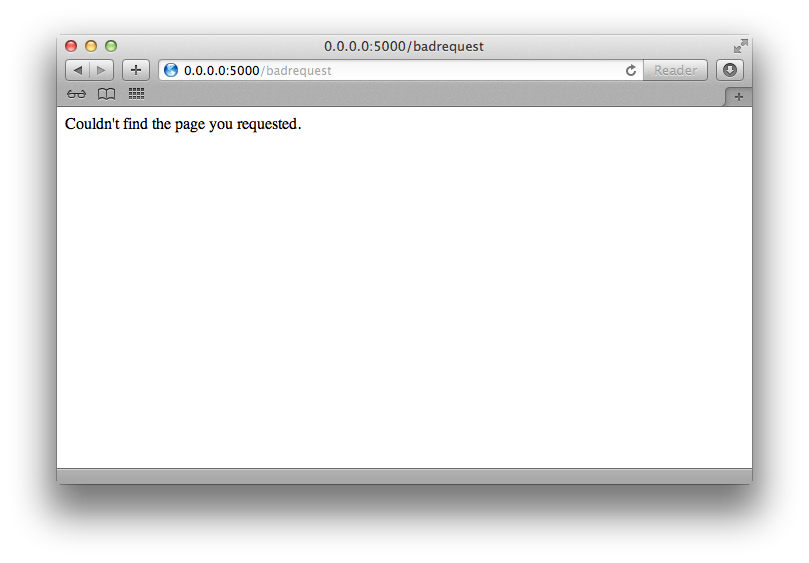
\includegraphics[width=0.9\textwidth]{images/flask-404-text.png}
\caption{The default 404 Not Found page}
\label{fig:flask-404-text}
\end{figure}

\paragraph{} Obviously this is not much better than the default but it does mean that we can start to build custom errors for our web-app, and once we start to look at returning HTML pages, using templates, and adding style with CSS then custom errors really become useful.

\paragraph{} You should also be aware that there are many error codes that your web-app might conceivably respond to. Some, badly designed sites will only respond with a 404 regardless of the error that occured, but the range of error codes actually means that you can respond with appropriate information that enables your user to make an informed decision about what to do next. Try implementing some other error codes. Because it can be difficult to force these errors to occur there is a shortcut in Flask that allows us to inject a specific type of error at any point which can be useful for testing.

\begin{lstlisting}
from flask import Flask, abort
app = Flask(__name__)

@app.route("/")
def hello():
  return "Hello Napier"

@app.route('/force404')
def force404():
  abort(404)

@app.errorhandler(404)
def page_not_found(error):
  return "Couldn't find the page you requested.", 404

if __name__ == "__main__":
  app.run(host='0.0.0.0', debug=True)
\end{lstlisting}

\paragraph{} Note the line that contains ``abort(404)''. In this line the abort function is used which immediately causes an error to occur resulting in the corresponding errorhandler being called.

\section{Flask Static Files}
\label{static}
\paragraph{} Even though we have seen some techniques for generating web-apps and pages dynamically from code, it is often useful to have static files, e.g. javascript, images, and CSS, that are stored in the filesystem. This enables you to incorporate useful standard web tools like, for example, JQuery, into your web-app, so you don't have to write \emph{everything} in Python.

\paragraph{} To use static files, all you have to do is to create directory called `\emph{static}' that is a sub-directory (child) of the directory in which your web-app is located. Notice that usually, if you were deploying your web-app in the wild as a public web-site then you would let your web-server take the load of hosting and serving up the files themselves and we will consider this approach later in the module\footnote{Deployment, hosting, administration, \& tuning of high-performance web sites is outside the scope of this module, and could alone form an entire module, however we will consider and discuss a range of tools and techniquess for deploying Flask web-apps that are generally applicable to most web sites.}. However, during development it is sufficient to use the \emph{static} sub-directory. You can then access the static file, for example a CSS file called \emph{style.css}, using theFlask url\_for function like so:

\begin{lstlisting}
    url_for('static', filename='style.css')
\end{lstlisting}

\paragraph{} NB. For this to work the file \emph{style.css} must be stored in the /static/ subdirectory. Here is full example that display an image in your browser. To get his to work you will have to create the /static/ directory then put an image file into it. You can use the curl tool at the command line to retrieve a remote image from the internet like so:

\begin{lstlisting}[style=DOS]
    $ curl siwells.github.io/assets/images/vmask.jpg -o vmask.jpg
\end{lstlisting}

\paragraph{} which will store an image file called \emph{vmask.jpg} in the directory in which the command is run. You can then use the following to display the file:

\begin{lstlisting}
from flask import Flask, url_for, abort
app = Flask(__name__)

@app.route("/")
def hello():
  return "Hello Napier"

@app.route('/static-example/img')
def static_example_img():
  start = '<img src="'
  url = url_for('static', filename='vmask.jpg')
  end = '">'
  return start+url+end, 200

if __name__ == "__main__":
  app.run(host='0.0.0.0', debug=True)
\end{lstlisting}

\paragraph{} Notice how we have used a standard HTML image (img) tag, filled in the src attibute using the output from url\_for, then concatenated the three strings together to form the string that is returned by the static\_example\_img function. I wonder what other HTML tags could be used to return information from a URL? Perhaps we could build entire web-pages this way, by just concatenating various sections of HTML to make an entire page....\footnote{You can do this, and you can return \emph{any} HTML tags this way and build up quite complex pages. However in chapter \ref{lab5} we will look at how we can use templates to design how our pages look using a mixture of HTML and special coding tags to dynamically build pure HTML responses.}.

\paragraph{} If you now visit \url{http://0.0.0.0:5000/static-example/img} you will see the relative URL for the image file something like this:

\begin{figure}[H]
\centering
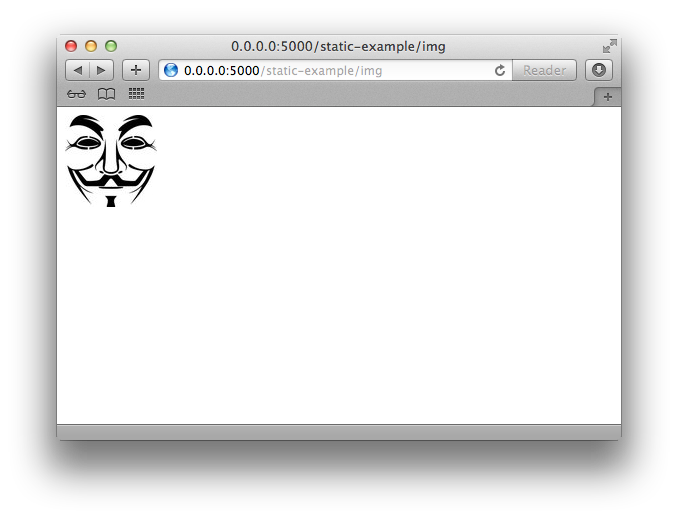
\includegraphics[width=0.9\textwidth]{images/flask-static-img.png}
\caption{Displaying a static image using the \emph{url\_for} function}
\label{fig:flask-static-img}
\end{figure}


%%%%%%%%%%%%%%%%%
%%%%%%%%%%%%%%%%%
% CHAPTER 04
%%%%%%%%%%%%%%%%%
%%%%%%%%%%%%%%%%%

\chapter{Python Flask: Requests \& Responses}
\label{lab04}
\paragraph{} In the last chapter we looked at how to do routing. That is how to execute a different function depending upon which URL the browser requested. This week we will look in more detail at the requests themselves. Because requests can include more than just a simple HTTP GET we shall look at how to handle different HTTP methods, such as GET, POST, PUT, \& DELETE, before looking at URL encoding of arguments to a route. The, after receiving and handling request data, we will look at the responses that we can return to the client.


\section{Requests}
\label{requests}
\paragraph{} When your browser connects to a URL it is making a {\textbf request}. In Flask, requests are Python objects that we can access and whose data we can reuse. For example, a request might carry a payload such as a document associated with a POST request and we will likely need to retrieve that payload document from the request in order to process the data and return an appropriate response.

\paragraph{} You can, for development, debugging, and educational purposes, investigate the request object by printing the request.method, request.path, and request.form attributes to retrieve data about the actual request, e.g.

\begin{lstlisting}
print request.method, request.path, request.form
\end{lstlisting}

\subsection{HTTP Methods}
\label{http-methods}
\paragraph{} HTTP uses various methods to move data around. The most commonly used method, and the one we have used exclusively until now is the default GET method. Look at the output from the Python Flask development server and you should see lines similar to the following:

\begin{lstlisting}[style=DOS]
10.0.2.2 - - [27/Sep/2015 18:59:51] "GET / HTTP/1.1" 200 -
10.0.2.2 - - [27/Sep/2015 18:59:58] "GET /hello HTTP/1.1" 200 -
10.0.2.2 - - [27/Sep/2015 19:00:05] "GET /goodbye HTTP/1.1" 200 -
\end{lstlisting}

\paragraph{} Notice the part of each line that says GET? This is because we have been interested only in retrieving information using the \emph{de facto} default HTTP method.
\paragraph{} HTTP specifies a range of methods for requesting web resources and these methods are oftern referred to as HTTP Verbs. By default a client usually makes GET requests and most web resources will respond to a GET request, however a resource, identified by a route, can respond differently to different verbs. So, for example, we can make a GET request to retrieve a resource or a POST request to send information to the resource. We can then write code to respond to differnt requests in different ways.

\paragraph{} As we said, a Flask route will accept GET requests by default, and Flask also supports HEAD requests automatically when GET is present, but we can also add support for other verbs to the route decorator method, e.g. to specify that a route can accept both GET and POST requests we would use the following decorator:

\begin{lstlisting}
@app.route('/account', methods=['GET', 'POST'])
\end{lstlisting}

\paragraph{} Within the method associated with that decorator we could then use an \emph{if...else} block to execute different code, e.g. 

\begin{lstlisting}
from flask import Flask, request
app = Flask(__name__)

@app.route("/")
def root():
  return "The default, 'root' route"

@app.route("/account/", methods=['GET', 'POST'])
def account():
  if request.method == 'POST':
    return "POST'ed to /account root\n"
  else:
    return "GET /account root"

if __name__ == "__main__":
  app.run(host='0.0.0.0', debug=True)
\end{lstlisting}


\paragraph{} To test this we can browse to \url{http://localhost:5000/account} and we should see the result of GET'ting the request.

\begin{figure}[H]
\centering
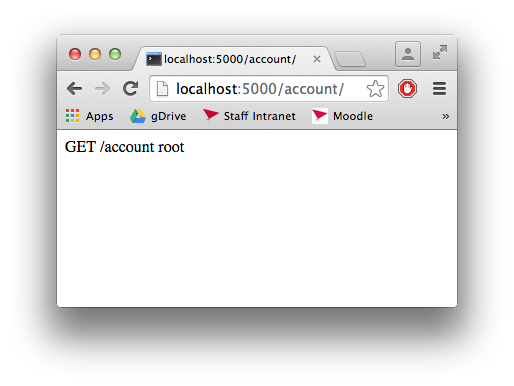
\includegraphics[width=0.9\textwidth]{images/flask-simple-posting.png}
\caption{Result from GET'ting our account/ route}
\label{fig:flask-simple-posting}
\end{figure}


\paragraph{} To test the POST call is slightly more involved for now. As we haven't implemented any HTML yet that is capable of calling this root using a POST request we need to mock one up. We can use cURL for that. The easiest way is to open a new SSH window and log in to your Levinux server then execute cURL locally on the server. We could do the same from Windows but working with the Windows command line is a pain (and we have already invested time in learning the Linux command line so we might as well continue with that. In Levinux you can now just run:

\begin{lstlisting}[style=DOS]
$ curl -i -X POST http://localhost:5000/account/
\end{lstlisting}

\paragraph{} Which will give output like this:

\begin{lstlisting}[style=DOS]
HTTP/1.0 200 OK
Content-Type: text/html; charset=utf-8
Content-Length: 24
Server: Werkzeug/0.10.4 Python/2.7.10
Date: Sun, 04 Oct 2015 12:51:12 GMT

POST'ed to /account root
tc@box:~$ 
\end{lstlisting}

\paragraph{} We can find out what HTTP method was used by checking the request method (as we saw in section \ref{http-methods}). Data transmitted in a POST or PUT request can then be accessed using the form attribute of the request object.

\subsection{Request \& Request Form Data}
\label{requests-objects-and-form-data}
\paragraph{} Now let's look at an example that displays a form when we connect to the URL using GET then display a different page that uses data from the form when we submit a POST request by pressing the form's button.

\begin{lstlisting}
from flask import Flask, request
app = Flask(__name__)

@app.route("/account/", methods=['POST','GET'])
def account():
  if request.method == 'POST':
    print request.form
    name = request.form['name']
    return "Hello %s" % name
  else:
    page ='''
    <html><body>
      <form action="" method="post" name="form">
        <label for="name">Name:</label>
        <input type="text" name="name" id="name"/>
        <input type="submit" name="submit" id="submit"/>
      </form>
      </body><html>'''

    return page
    
if __name__ == "__main__":
  app.run(host='0.0.0.0', debug=True)
\end{lstlisting}

\paragraph{} This should yield something similar to the following when we visit \url{http://localhost:5000/account/} in the browser:

\begin{figure}[H]
\centering
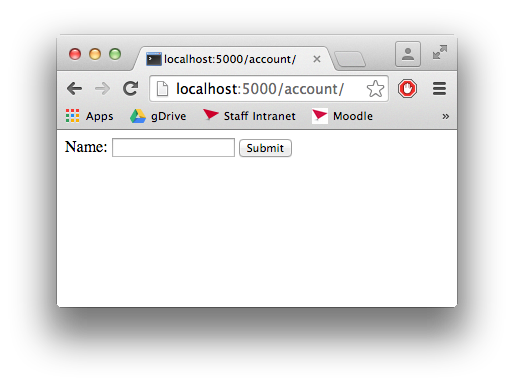
\includegraphics[width=0.9\textwidth]{images/flask-form.png}
\caption{Our basic HTML form when GET'ting the account route}
\label{fig:flask-form}
\end{figure}

\paragraph{} It is worth noting how we have used a Python multiline string, which starts with ''' and ends with ''' to build up an html page completely within out Python function. When we enter data into the input box the click the button we should get different page displayed as a result of the form POST'ing:

\begin{figure}[H]
\centering
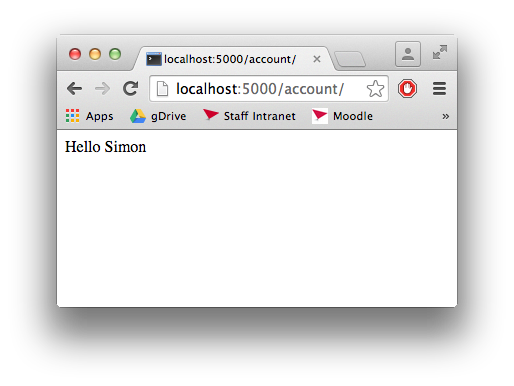
\includegraphics[width=0.9\textwidth]{images/flask-form-data.png}
\caption{Page displayed after POST'ing the form}
\label{fig:flask-form-data}
\end{figure}



\paragraph{} We will return to using POST, PUT, and other verbs in chapter \ref{lab08} when we look at designing and building APIs that consume and return JSON and XML documents.


\subsection{URL Variables}
\label{url-variables}
\paragraph{} We can also construct URLs that have variables within them. For example, if we wanted a URL route that enabled us to retrieve a user's details by name then we might want a URL of the following pattern \emph{/account/$<$username$>$} where $<$username$>$ is replaced by an actual name. We can achieve this using URL variables, e.g.

\begin{lstlisting}
from flask import Flask
app = Flask(__name__)

@app.route("/hello/<name>")
def hello(name):
  return "Hello %s" % name

if __name__ == "__main__":
  app.run(host='0.0.0.0', debug=True)
\end{lstlisting}

\paragraph{} We can now call the url, e.g. using the name 'simon' in the following \url{http://localhost:5000/hello/simon} and we would get the following output:

\begin{figure}[H]
\centering
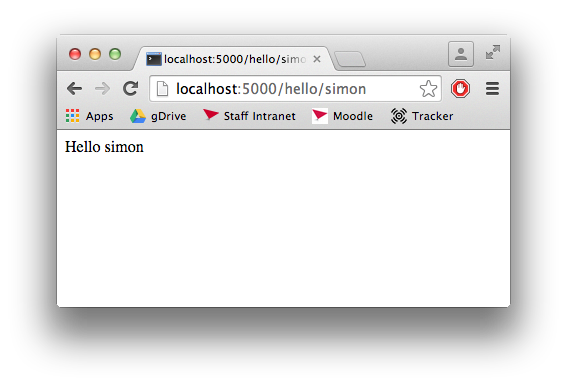
\includegraphics[width=0.9\textwidth]{images/flask-url-variables.png}
\caption{Using URL variables}
\label{fig:flask-url-variables}
\end{figure}

\paragraph{} By default URL variable are strings but we ca also specify other variable types such as int and floats, for example,

\begin{lstlisting}
from flask import Flask
app = Flask(__name__)

@app.route("/add/<int:first>/<int:second>")
def add(first, second):
  return str(first+second)

if __name__ == "__main__":
  app.run(host='0.0.0.0', debug=True)
\end{lstlisting}

\paragraph{} With the following result:

\begin{figure}[H]
\centering
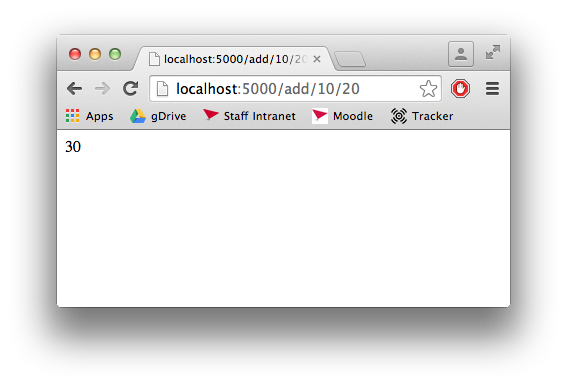
\includegraphics[width=0.9\textwidth]{images/flask-url-variables-ints.png}
\caption{Output from using specific URL variable types}
\label{fig:flask-url-variables-ints}
\end{figure}



\subsection{URL Parameters}
\label{url-parameters}
\paragraph{} Rather than construct and send a document to the server or use a POST'ed form, we will often want to send small amount of non-secure data to the server encoded within the URL. This is straightforward in Flask. 

\paragraph{} Parameters can be encoded in the URL when a client make a request. Flask can retrieve these parameters and use them by using the args attribute of the request object, e.g. for a URL that incorporates \emph{?key=value} parameters similar to the following:

\begin{lstlisting}[style=DOS]
/update?colour=green
\end{lstlisting}

\paragraph{} Then we can access the corresponding keys like so:

\begin{lstlisting}
searchterm = request.args.get('key', '')
\end{lstlisting}

\paragraph{} The value for key is then retrieved from the URL and stored in `searchterm'. If no such key is supplied then the value in the second pair of quotes is used as a default instead but in the example above we have just used an empty string.

\paragraph{} Now let's look at a simple example, which you can use to send your name as a URL encoded parameter, and have a route accept and process it we can do the following:

\begin{lstlisting}
from flask import Flask, request
app = Flask(__name__)

@app.route("/hello/")
def hello():
  name = request.args.get('name', '')
  if name == '':
    return "no param supplied"
  else:
    return "Hello %s" % name

if __name__ == "__main__":
  app.run(host='0.0.0.0', debug=True)
\end{lstlisting}

\paragraph{} When we run this without supplying a parameter, e.g \url{http://localhost:5000/hello/} then we get this output:

\begin{figure}[H]
\centering
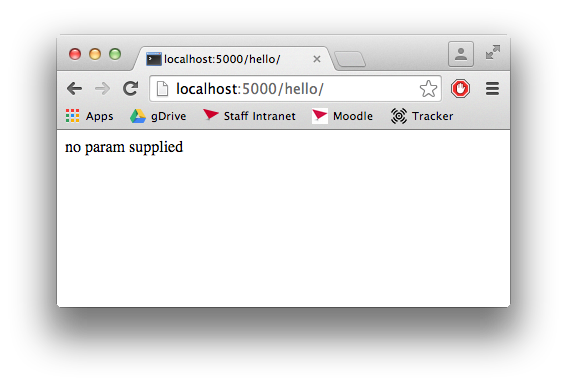
\includegraphics[width=0.9\textwidth]{images/flask-url-param-empty.png}
\caption{Output with no URL parameter}
\label{fig:flask-url-param-empty}
\end{figure}

\paragraph{} When we supply a parameter, e.g. \url{http://localhost:5000/hello/?name=simon} then we get this output:

\begin{figure}[H]
\centering
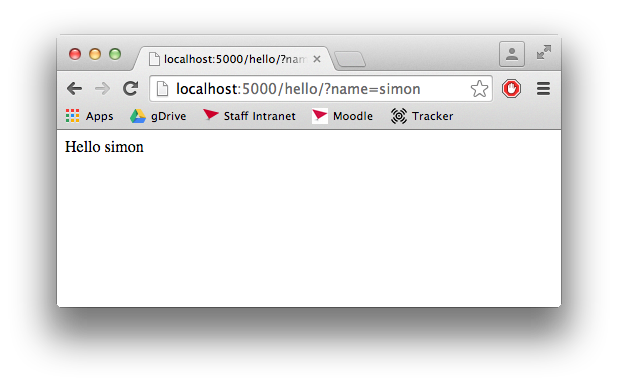
\includegraphics[width=0.9\textwidth]{images/flask-url-param-name.png}
\caption{Output when supplying a ?name=simon URL parameter}
\label{fig:flask-url-param-name}
\end{figure}


\subsection{Uploading Files}
\label{file-uploading}
\paragraph{} One final thing to consider that is related to client requests, is the matter of file uploading. We will occasionally want to enable our users to upload materials to our site and we can do this by ensuring that two things occur. The form which POSTs the data must cause the browser to transmit the file that we want to upload and our method that the route executes must also access the request and do something with the transmitted file. Otherwise the file will sit by default either in memory or in temptorary storage rather then being saved for later reuse. In the following I used a PNG image file that I had available as the uploaded file:

\begin{lstlisting}
from flask import Flask, request
app = Flask(__name__)

@app.route("/account/", methods=['POST','GET'])
def account():
  if request.method == 'POST':
    f = request.files['datafile']
    f.save('static/uploads/upload.png')
    return "File Uploaded"
  else:
    page='''
    <html>
    <body>
    <form action="" method="post" name="form" enctype="multipart/form-data">
      <input type="file" name="datafile" />
      <input type="submit" name="submit" id="submit"/>
    </form>
    </body>
    </html>
    '''
    return page, 200

if __name__ == "__main__":
  app.run(host='0.0.0.0', debug=True)
\end{lstlisting}

\paragraph{} Notice that the file is being saved in a sub-directory of static called `uploads'. This makes it easier to access the uploaded file and use it within our app. Look in `static/uploads' for the new file. Perhaps you could combine this file upload facility with the image display example that we saw in section \ref{static}. For example:

\begin{lstlisting}
from flask import Flask, request, url_for
app = Flask(__name__)

@app.route("/display/")
def display():
  return '<img src="'+url_for('static', filename='uploads/file.png')+'"/>'

@app.route("/upload/", methods=['POST','GET'])
def account():
  if request.method == 'POST':
    f = request.files['datafile']
    f.save('static/uploads/file.png')
    return "File Uploaded"
  else:
    page='''
    <html>
    <body>
    <form action="" method="post" name="form" enctype="multipart/form-data">
      <input type="file" name="datafile" />
      <input type="submit" name="submit" id="submit"/>
    </form>
    </body>
    </html>
    '''
    return page, 200

if __name__ == "__main__":
  app.run(host='0.0.0.0', debug=True)
\end{lstlisting}

\paragraph{} Of interest here is that when we access the display method repeatedly you should see in the output from the Flask development server something similar to this:

\begin{lstlisting}[style=DOS]
10.0.2.2 - - [05/Oct/2015 17:29:14] "GET /display/ HTTP/1.1" 200 -
10.0.2.2 - - [05/Oct/2015 17:29:15] "GET /static/uploads/file.png HTTP/1.1" 304
\end{lstlisting}

\paragraph{} In this case we get the 304 because the image file hasn't changed (another reason we store it in our static repository. However, a final note on file uploads and static files. In a real-world deployment we usually wouldn't serve static files directly from within Flask as other HTTP servers like NGinX can do this much more reliably and efficiently. However for development and educational purposes using the Flask static directory is an acceptable approach.


\section{Responses}
\label{responses}
\paragraph{} When we return a value from a function it is automatically turned into a valid HTML response object. If the value is a String then it is used as the body of the response which is why when we just do something like this:

\begin{lstlisting}
from flask import Flask
app = Flask(__name__)

@app.route("/")
def root():
    return "Hello Napier"

if __name__ == "__main__":
  app.run(host='0.0.0.0', debug=True)
\end{lstlisting}

\paragraph{} then our browser displays the String that the function returned. A 200/OK HTTP status code is also returned by default and the mimetype is set to text/html. We will return to this topic later when we look at API building and consider setting and returning custom headers.



%%%%%%%%%%%%%%%%%
%%%%%%%%%%%%%%%%%
% CHAPTER 05
%%%%%%%%%%%%%%%%%
%%%%%%%%%%%%%%%%%
\chapter{HTML Templates using Jinja2}
\label{lab05}
\paragraph{} Storing and writing our HTML code in Python as we have done in previous chapters is not a lot of fun. It is finicky and error-prone and doesn't give us much scope for doing interesting things like generating HTML pages on the fly. Luckily there is a solution for that. Using \emph{templates} we can describe the basic layout of a page and sign-post those elements that Python can fill in with actual data. Python uses an external templating engine, called Jinja2\footnote{\url{http://jinja.pocoo.org/2/}} which is already installed in Levinux alongside Python and Python-Flask.

\paragraph{} Jinja2 is a fully-fledged Python templating engine and is not dependent upon Flask. So if you were writing another app at some point in your career that outputs HTML pages then Jinja2 is a good option. For the moment though we shall use it exclusively with Flask.


\subsection{Templates \& Tags}
\label{templates-tags}
\paragraph{} The process is simple. We supply HTML templates, in a template folder, then, in our functions we tell Flask which template to render and return to the client using the render\_template function. So we have a couple of setup tasks to do. First, create a templates folder in the same folder as your Python Flask app, e.g.

\begin{lstlisting}[style=DOS]
$ mkdir templates
\end{lstlisting}

\paragraph{} Now create a simple HTML template, called hello.html inside the templates folder, e.g.
\begin{lstlisting}[style=DOS]
$ touch templates/hello.html
\end{lstlisting}

\paragraph{} Now open hello.html in Vim for editing, e.g.
\begin{lstlisting}[style=DOS]
$ vim templates/hello.html
\end{lstlisting}

\paragraph{} Now we can put some HTML and Jinja2 tags into our template so that we can use the template from within Flask:


\begin{lstlisting}
<!doctype html>
    <h1>Hello {{ user.name }}!</h1>
</html>
\end{lstlisting}

\paragraph{} What we have just done is create a template that is a mix of Jinja2 tags, indicated by the \{\{, and \}\} tags, and HTML tags, indicated by the $<$ and $>$ tags that we are already used to. The HTML tags are rendered as you would expect regular HTML to be treated, but we also have a variable placeholder for user.name which means that we can supply a variable to replace the name placeholder with. Let's use our template now in a quick Flask app:

\begin{lstlisting}
from flask import Flask, render_template
app = Flask(__name__)

@app.route('/hello/<name>')
def hello(name=None):
    user = {'name': name}
    return render_template('hello.html', user=user)

if __name__ == "__main__":
    app.run(host='0.0.0.0', debug=True)
\end{lstlisting}

\paragraph{} Now if we call \url{localhost:5000/hello/simon} then we should instead see this rendered template:

\begin{figure}[H]
\centering
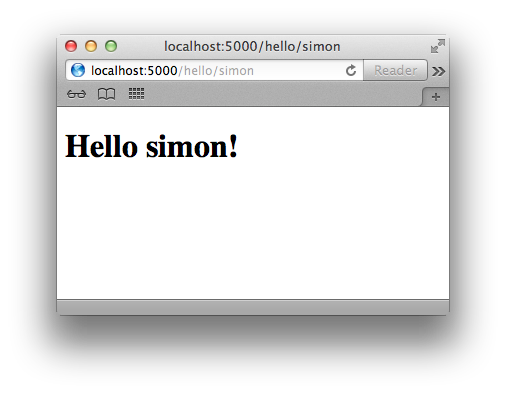
\includegraphics[width=0.9\textwidth]{images/flask_template_basic}
\caption{Rendered HTML with a very simple template \& a single parameter}
\label{fig:flask_template_basic}
\end{figure}


\subsection{Templates with Conditional Arguments}
\label{templates-conditional}
\paragraph{} We can also use Jinja2 templates to perform conditional behaviours, for example, rendering our HTML differently depending upon the data that is passed in. This lets us do things like personalise a page if we have a person's name or else provide a default generic page if we don't. Let's look at the template (conditional.html) for such a scenario:

\begin{lstlisting}
<!doctype html>

    <h1>Hello {{ name }}!</h1>

    <h1>Hello from Napier!</h1>

</html>
\end{lstlisting}

\paragraph{} The Jinja2 tags cause conditional behaviour to occur; in this case they form an if...else clause, just like we have seen in many other procedural languages like Java, C, or even Python. Let's use our template now in a quick Flask app:

\begin{lstlisting}
from flask import Flask, render_template
app = Flask(__name__)

@app.route('/hello/')
@app.route('/hello/<name>')
def hello(name=None):
    return render_template('conditional.html', name=name)

if __name__ == "__main__":
    app.run(host='0.0.0.0', debug=True)
\end{lstlisting}

\paragraph{} There are a couple of things to notice here:
\begin{enumerate}
\item Notice how we have stacked up two @app.route calls - yes, a single function can have multiple routes defined for it, any of which can cause the function to be executed.
\item We have also used a URL variable in one of the route so that we can supply a name. Notice that the hello function takes a name argument and that it is set to `name=None' - this just means that we have set a default value for name in case the route without the URL variable is used.
\item In the hello function we use the render\_template function from the Flask library which basically looks in the templates directory for a template whose name matched the one that we have supplied, `hello\_template.html'. The function then \emph{completes} the template, i.e. exchanging the Jinja2 tags for valid HTML tags, according to the arguments that we provide. In this case we provide the name=name argument, which will either have the value of None or else will be equal to the name that we supplied when we called the route. This argument is used to determine which path of the if...else clause to follow in the template and what value to replace any template variables with.
\end{enumerate}

\paragraph{} If we now call \url{localhost:5000/hello} then we should see the following:

\begin{figure}[H]
\centering
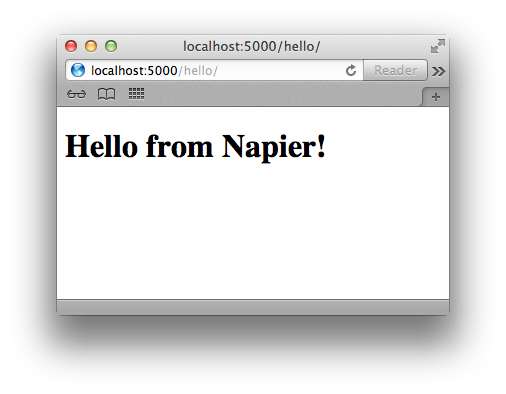
\includegraphics[width=0.9\textwidth]{images/flask-template-conditional-no-arg}
\caption{Conditional template rendering without URL arguments}
\label{fig:flask-template-conditional-no-arg}
\end{figure}

\paragraph{} But if we call \url{localhost:5000/hello/simon} then we should instead see this rendered template:

\begin{figure}[H]
\centering
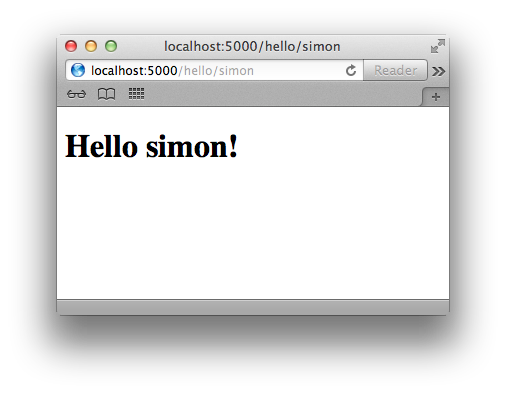
\includegraphics[width=0.9\textwidth]{images/flask-template-conditional-arg}
\caption{Conditional template rendering with a single URL argument}
\label{fig:flask-template-conditional-arg}
\end{figure}


\subsection{Templates \& Collections}
\label{templates-collections}
\paragraph{} A very useful technique for generating HTML is to build a list or dictionary in Python then pass that collection into the template and cause the template to iterate over the elements of the collection. Let's look at a simple example now; here is a simple template that incorporates a Jinja2 looping construct:

\begin{lstlisting}
<!doctype html>
<body>
  <ul>
    
     <li>{{ name }}</li>
    
  </ul>
</body>
</html>
\end{lstlisting}

\paragraph{} We can now use this template in a Python Flask function as illustrated here:

\begin{lstlisting}
from flask import Flask, render_template
app = Flask(__name__)

@app.route('/users/')
def users():
  names = ['simon', 'thomas', 'lee', 'jamie', 'sylvester']
  return render_template('loops.html', names=names)

if __name__ == "__main__":
  app.run(host='0.0.0.0', debug=True)
\end{lstlisting}

\paragraph{} Notice that we merely constructed a Python list, a simple data structure, that is a list of names. We then passed that list into the render\_template function for processing by the templating engine. If we now visit \url{localhost:5000/users/} we should see that our Python list has been rendered as an unordered HTML list.

\begin{figure}[H]
\centering
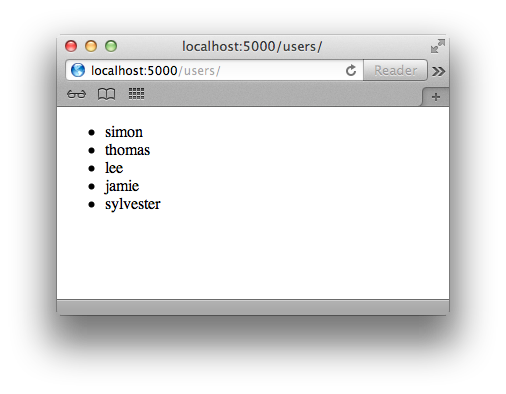
\includegraphics[width=0.9\textwidth]{images/flask-templates-loops}
\caption{Looping over data in within a template to generate HTML}
\label{fig:flask-templates-loops}
\end{figure}

\paragraph{} By using simple looping techniques and carefully considering the data that we pass from our Python function into a template, we can generate complex and dynamic HTML layouts.


\subsection{Template Inheritance}
\label{template-inheritance}
\paragraph{} Because multiple templates can also be used to define headers, footers, and any other sub-part of individual pages in your app this means you can easily change and manage the look and feel of your apps. This approach is called \emph{Template Inheritance} and means that you can, for example, define a header or menu-bar just once, e.g. in a template called menu.html and then include that template in every other pages which you want to display the menu. If you ever wish to add or remove a menu item then you only have to make a single edit to the menu template. Nice isn't it? This follows an established software design pattern of attempting to separate application logic separate from the presentation, markup or layout of data. Although you might ask, ``what about the logic in the template?'', you are correct, there is a little bit of overlap where logic directly concerns rendering the templates but for the most part, done correctly, all of the computation of your web-app should be done in Flask and the rendering into HTML is done separately in Jinja2. This is a pretty good balance I think.

\paragraph{} To demonstrate template inheritance we will first define a base template, then two templates that inherit from it. We will then create some routes that render the templates. So let's start with our base template:

\begin{lstlisting}
<html>
<head>
    <title>Template Inheritance Example</title>
</head>
<body>
    <h1>Title stored in the base template</h1>
    <h2>With a subtitle</h2>

     

</body>
</html>
\end{lstlisting}

\paragraph{} For the most part this is just a normal HTML file except that it incorporates some Jinja2 tags to set out blocks that we have called `content'. It is these blocks that are replaced within the templates that inherit from the base template. We can now inherit this base template and reuse the common elements as follows:

\begin{lstlisting}


  <p>First example template. It contains some stuff</p>
}
\end{lstlisting}

\paragraph{} The main point to be aware of is that the \emph{derived} template specifies that it inherits from the base template. Just to demonstrate that this works for different templates, let's create a second template that also inherits from the base template but which contains different content to the last pone.

\begin{lstlisting}


  <p>A second example. It's different to the other one.</p>
}
\end{lstlisting}

\paragraph{} We can make a Flask file which has routes that render our templates.

\begin{lstlisting}
from flask import Flask, render_template
app = Flask(__name__)

@app.route('/inherits/')
def inherits():
    return render_template('base.html')

@app.route('/inherits/one/')
def inherits_one():
    return render_template('inherits1.html')

@app.route('/inherits/two/')
def inherits_two():
    return render_template('inherits2.html')

if __name__ == ("__main__"):
    app.run(host='0.0.0.0', debug=True)
\end{lstlisting}

\paragraph{} Here we have three different routes. The first one `/inherits/' merely shows what the base template looks like when it is rendered without additional templates that inherit from it. In the other two routes `/inherits/one/' and `/inherits/two/' we see how the base template is modified when it is extended by two different inheriting templates. Using this approach we can build a hierarchy of page templates whilst minimising the amount of reptition by ensuring that each element that will be repeated between HTML pages is inherited from a parent template.

\paragraph{} This is the output from our first template that inherits from base.html. It displays some content that comes from inherits1.html and some headings that are inherited from the base template.

\begin{figure}[H]
\centering
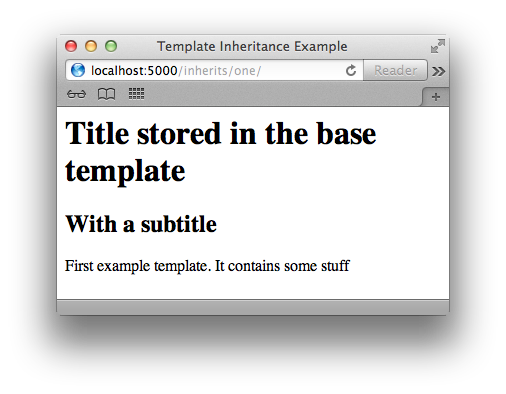
\includegraphics[width=0.9\textwidth]{images/flask-template-inheritance-1}
\caption{The first page that inherits from our base template}
\label{fig:flask-template-inheritance-1}
\end{figure}

\paragraph{} Our second page that inherits from the base template. Notice that the same headers are displayed as on the other page. However we have different content as defined by the inherits2.html template.

\begin{figure}[H]
\centering
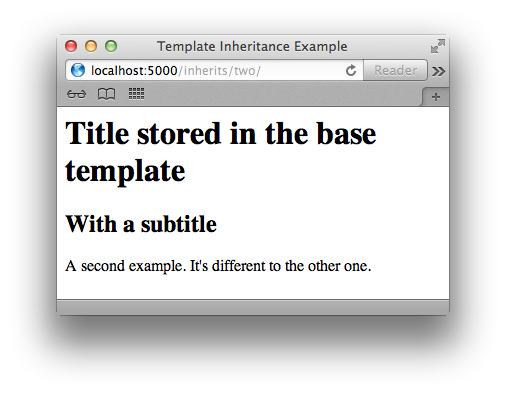
\includegraphics[width=0.9\textwidth]{images/flask-template-inheritance-2}
\caption{The second page that inherits from our base template}
\label{fig:flask-template-inheritance-2}
\end{figure}

\paragraph{} Just for completion, let's also look at what the base template looks like when rendered. We don't \emph{have} to provide a route to it, but if we do then we can view the HTML that it generates:

\begin{figure}[H]
\centering
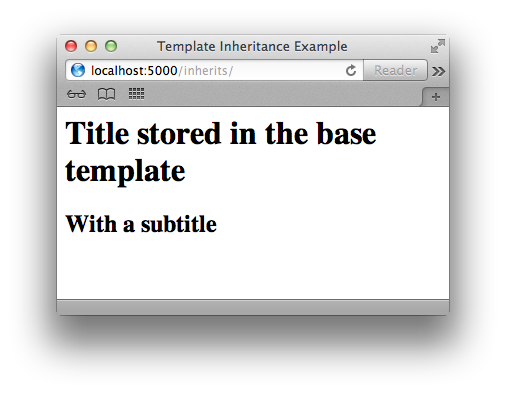
\includegraphics[width=0.9\textwidth]{images/flask-template-inheritance-base}
\caption{The rendered base template}
\label{fig:flask-template-inheritance-base}
\end{figure}

\paragraph{} You can and should use templates to describe all of the HTML pages that you want your web-apps to use. This approach is a consistent and very powerful method for generating HTML and managing the look of your web-apps.


%%%%%%%%%%%%%%%%%
%%%%%%%%%%%%%%%%%
% CHAPTER 06
%%%%%%%%%%%%%%%%%
%%%%%%%%%%%%%%%%%
%\begin{comment}
\chapter{Flask: Configs, Sessions, Message Flashing, Logging, \& Testing}
\label{lab06}
\paragraph{} 

\section{Configuration \& Config Files}
\label{configs}
\paragraph{} Quite often we need to do external configuration of our Flask app, for example, if we are using external tools, like Babel, to control translations into different languages, if we need to specify an encryption key for setting up secure sessions, or a password for accessing an external mail server. We can achieve this by using configuration files, external text files that Flask can read at start up and which provide data to Flask about the environment it is running in.

\paragraph{} Create a sub-directory called `etc' just like you did for the static and templats directories. Your config files will live here. Now create a new text file in the etc directory called `defaults.cfg', this will be the default file that your flask app reads in at start up. We can now use that file to store some configuration data. Let's start by moving our debug and host settings into the config file instead of setting them in code, e.g. Add the following to your defaults.cfg:

\begin{lstlisting}
[config]
debug =  True
ip_address = 0.0.0.0
port = 5000
url = http://127.0.0.1:5000
\end{lstlisting}

\paragraph{} Our config file can be used to store whichever configuration values we decide we want to support in a flask app. For illustration purposes I have used the debug flag na ip, url, port numbers settings. We can now create a Flask app that uses those values, for example,

\begin{lstlisting}
import ConfigParser

from flask import Flask

app = Flask(__name__)

@app.route('/')
def root():
  return "Hello Napier from the configuration testing app"

@app.route('/config/')
def config():
  str = []
  str.append('Debug:'+app.config['DEBUG'])
  str.append('port:'+app.config['port'])
  str.append('url:'+app.config['url'])
  str.append('ip_address:'+app.config['ip_address'])
  return '\t'.join(str)

def init(app):
    config = ConfigParser.ConfigParser()
    try:
        config_location = "etc/defaults.cfg"
        config.read(config_location)
        
        app.config['DEBUG'] = config.get("config", "debug")
        app.config['ip_address'] = config.get("config", "ip_address")
        app.config['port'] = config.get("config", "port")
        app.config['url'] = config.get("config", "url")
    except:
        print "Could not read configs from: ", config_location

if __name__ == '__main__':
    init(app)
    app.run(
        host=app.config['ip_address'], 
        port=int(app.config['port']))
\end{lstlisting}

\paragraph{}  Notice how we are `getting' the value for each key from the config file then storing those values in the app.config object. 

\section{Sessions}
\label{sessions}
\paragraph{} Sessions are a way to manage user data between requests by storing small amounts of data within a cookie. Cookies are small data files that are stored in the users browser and are suitable for small amounts of, ideally non-private, data. Sessions rely on cookies that are cryptographically secured by Flask using a secret key to ensure that the content of the cookies hasn't been altered by any process other than the Flask app that created it. However, the content of a cookie can easily be read by the client or whilst it is transmitted between the client and server during a request\footnote{Unless the communication has been secured with HTTP but that is another topic}.

\paragraph{} Flask provides an interface for using `secured cookies' or \emph{sessions} rom our Python code and we can consider a session to be a small data store for keys and value, a form of dictionay. As a result we can set data into a session, query that data, and remove that data, 

\paragraph{} To add a key value pair we merely treat the session object as a Python dictionary\footnote{If you are unsure about Python dictionaries or `dicts' then you should do some background reading on this topic in the Python language documentation}, e.g.
\begin{lstlisting}
# Set key=value, name=simon into a session
session['name'] = simon
\end{lstlisting}

\paragraph{} You can then retrieve the value set for name in the session but because this key might not exist in the session we need to wrap everything in a try-except structure to catch the KeyError that might be raised\footnote{Again, if you are unsure about Python errors \& try-execept then you should do background reading on this}.
\begin{lstlisting}
try:
    if(session['name']):
        return str(session['name'])
except KeyError:
    pass
\end{lstlisting}

\paragraph{} The only other thing that we might need to do is to remove a specified key and it's associated value from the session. We do this using the pop function, e.g.
\begin{lstlisting}
session.pop('name', None)
\end{lstlisting}

\paragraph{} We can then put it all together into a single demonstration web-app like so.

\begin{lstlisting}
from flask import Flask, session

app = Flask(__name__)
app.secret_key = 'A0Zr98j/3yX R~XHH!jmN]LWX/,?RT'

@app.route('/')
def index():
    return "Root route for the sessions example"

@app.route('/session/write/<name>/')
def write(name=None):
    session['name'] = name
    return "Wrote %s into 'name' key of session" % name

@app.route('/session/read/')
def read():
    try:
      if(session['name']):
          return str(session['name'])
    except KeyError:
      pass
    return "No session variable set for 'name' key"

@app.route('/session/remove/')
def remove():
    session.pop('name', None)
    return "Removed key 'name' from session"

if __name__ == "__main__":
  app.run(host='0.0.0.0', debug=True)
\end{lstlisting}

\paragraph{} Notice the `app.secret\_key' line. This is our secret key that is used to secure our session cookie so should really be stored securely, either in a config file or typed in by hand at startup, but never put in the code repository. However for demonstration purposes this is sufficient for now. The key above is sufficient for the lab work but you would generate a unique key for any real deployment and would keep it secret. You can generate a key easily using Python. Start the Python interpreter and use the os.urandom function to generate a new key that you can then copy and paste into your Flask app, e.g.

\begin{lstlisting}
$ Python
...
>>> import os
>>> os.urandom(24)
'\xfd{H\xe5<\x95\xf9\xe3\x96.5\xd1\x01O<!\xd5\xa2\xa0\x9fR"\xa1\xa8'
\end{lstlisting}


\section{Message Flashing}
\label{message-flashing}
\paragraph{} User feedback is an important consideration when trying to design a good user experience (UX). Message flashing is just one aspect of UX that Flask provides to enable easy user feedback. The scenario is quite simple, when the user does something on one page, which causes another page to be rendered and displayed, then information, a message, can be transmitted from the first page to the second, and displayed, e.g. flashed, to the user. This means that, used with the correct combinations of responses, users can interact with your web app and get feedback about the outcome of actions. A simple example will illustrate this; if you have a sign-up page for new users on which the user enters information then presses a ``join'' button you can use message flashing to provide a personalised message to the user on the next page that is displayed. For example, after pressing ``join'' either the sign up page will be redisplayed, because the supplied information is insufficient, or else the login page will be displayed. A flashed message could be displayed in either case, on the sign-up page to indicate what needs to be fixed, or on the log in page indicating that a new account was created and that the user is welcome to log in. What is essentially happening is that a message is recorded at the end of the first request, which is then accessed \emph{only} on the very next request.

\paragraph{} Message flashing sounds quite complex and does have a few moving parts, but is really very simple once you have used it once to twice. It is best shown via example, so let's get started with one

\begin{lstlisting}
from flask import Flask, flash, redirect, request, url_for, render_template

app = Flask(__name__)
app.secret_key = 'supersecret'

@app.route('/')
def index():
    return render_template('index.html')

    return "Root Page"

@app.route('/login/<message>')
def login(message):
    if (message != None):
      flash(message)
    flash("A default message")
    return "Let's pretend you just logged in"

if __name__ == "__main__":
    app.run(host='0.0.0.0', debug=True)
\end{lstlisting}
\paragraph{} Here, we have added a flashed message in one route, using the flash() function of Flask then we use the get\_flashed\_messages() method in our template to retrieve the flashed message and display it, e.g.

\begin{lstlisting}
<html>
<body>

  
    <ul>
    
      <li>{{ message | safe}}</li>
    
    </ul>
  

</body>
</html>
\end{lstlisting}

\paragraph{} All that we have done here is add a flashed messagein the `/login/$<$message$>$' route then to display the flashed message when we visit the `/' page. Subsequent visits to the `/' page will not repeat the flashed message, unless of course, we visit the `login/$<$message$>$' page again

\section{Logging}
\label{logging}
\paragraph{} We can set our Flask app up to record interesting happenings into a text file so that we have a log to inspect if something bad occurs. This is actually a feature of the Python language rather than a Flask feature, but is an important part of building a real world app. First we need to make some additions to our config file, e.g.

\begin{lstlisting}
[loggingapp]
debug =  True
ip_address = 0.0.0.0
port = 5000
url = http://127.0.0.1:5000
[logging]
name = loggingapp.log
location = var/
level = DEBUG
\end{lstlisting}
\paragraph{} Notice the logging section towards the end which defines the name of the log file `'loggingapp.log' the location, our var/ directory that we just created, and the default log level, the granularity of the logging events to record. 
\paragraph{} We now need to set up our envionrment to match the config file. We need a subdirectory called `var' which is at the same level as our `etc', `static' and `templates' directories. We now need to create an empty file in `var' which has the same name as the log file. This directory will be the location that our new log files will write to. We can do this with touch, e.g.

\begin{lstlisting}[style=DOS]
    $ mkdir var
    $ touch var/loggingapp.log
\end{lstlisting}

\paragraph{} Having set everything up all the configuration details and the basic environment we now need to make use of that set up within our python app:

\begin{lstlisting}
import ConfigParser
import logging

from logging.handlers import RotatingFileHandler
from flask import Flask, url_for

app = Flask(__name__)

@app.route('/')
def root():
        this_route = url_for('.root')
        app.logger.info("Logging a test message from "+this_route)
        return "Hello Napier from the configuration testing app (Now with added logging)" 

def init(app):
    config = ConfigParser.ConfigParser()
    try:
        config_location = "etc/logging.cfg"
        config.read(config_location)
        
        app.config['DEBUG'] = config.get("config", "debug")
        app.config['ip_address'] = config.get("config", "ip_address")
        app.config['port'] = config.get("config", "port")
        app.config['url'] = config.get("config", "url")

        app.config['log_file'] = config.get("logging", "name")
        app.config['log_location'] = config.get("logging", "location")
        app.config['log_level'] = config.get("logging", "level")
    except:
        print "Could not read configs from: ", config_location


def logs(app):
    log_pathname = app.config['log_location'] + app.config['log_file']
    file_handler = RotatingFileHandler(log_pathname, maxBytes=1024* 1024 * 10 , backupCount=1024)
    file_handler.setLevel( app.config['log_level'] )
    formatter = logging.Formatter("%(levelname)s | %(asctime)s |  %(module)s | %(funcName)s | %(message)s")
    file_handler.setFormatter(formatter)
    app.logger.setLevel( app.config['log_level'] )
    app.logger.addHandler(file_handler)

if __name__ == '__main__':
    init(app)
    logs(app)
    app.run(
        host=app.config['ip_address'], 
        port=int(app.config['port']))
\end{lstlisting}
\paragraph{} The init function is very similar to the one we used earlier in the config example but is now extended to also configure event logging. There are many parameters to fine tune how data is logged so if you want to make changes then you will have to dig into the Python logging documentation but for now, just accept the defaults as they produce files that cope well with lots of data, are easy to read, and which can be automatically processed. All we have had to do to use the logger is to initialise the logging system by calling our configuration modules logs() function. From then on we can actually log messages using the app.logger.warn() and passing in a String. NB. There are also other logging levels such as debug or error that we can use to distinguish the importance of different messages in the logs. Investigate the Python logging documentation to find out more. 

\paragraph{} Now, if everything is set up correctly, then every time we visit \url{http://localhost:5000/} a new log file should be added to var/loggingapp.log and we can use an extra PuTTY window to ``tail'' the log so that we see each new log line appear in realtime. Tailing a log just means to show the last entries in the file and using the `-f' argument to the tail command causes it to follow the log, meaning that each new line is displayed in the terminal like so:

\begin{lstlisting}[style=DOS]
tc@box:~$ tail -f var/loggingapp.log 
INFO | 2015-10-13 17:44:37,368 |  logs | root | Logging a test message from /
INFO | 2015-10-13 17:44:45,104 |  logs | root | Logging a test message from /
INFO | 2015-10-13 17:44:46,325 |  logs | root | Logging a test message from /
^C
tc@box:~$ 
\end{lstlisting}

\paragraph{} From this we can see that there were three log messages displayed and that the output is arranged into columns. Getting the output nice and neat like this is the main reason we had to write so much code in our python app and config file, but it is really worth it when you are trying to track down a problem.

\paragraph{} It is a good idea to log anything that you think that you might want to have a record of and that you might need to look up in order to bug fix. Unfortunately though there are no rules for what to log and what not to log. Obviously you could log \emph{everything} but this would possibly waste disk space, but not logging enough might mean that you don't have sufficient logs to help you fix problems. However, with experimentation and experience you will develop skills in gauging the right amount of and type of data to log.

\section{Testing}
\label{testing}
\paragraph{} We can unit test our Python app, to ensure that everything is working correctly. We do this by running a test harness which sets up our Flask app then compares expected outputs to actual outputs, for example, for the following simple web-app:

\begin{lstlisting}
from flask import Flask
app = Flask(__name__)

@app.route('/')
def root():
  return "HELLO NAPIER", 200

if __name__ == "__main__":
  app.run(host='0.0.0.0',debug=True)
\end{lstlisting}

\paragraph{} We can write tests that compare the response returned by a call to the `/' route against what we would expect. For example, is the content correct, is the content type set corretly, is the status value set correctly. Let's see some of these tests now.

\begin{lstlisting}
import unittest
import testing

class TestingTest(unittest.TestCase):
  def test_root(self):
    self.app = testing.app.test_client()
    out = self.app.get('/')
    assert '200 OK' in out.status
    assert 'charset=utf-8' in out.content_type
    assert 'text/html' in out.content_type

if __name__ == "__main__":
  unittest.main()
\end{lstlisting}

\paragraph{} We have create a class for the test and asserted that the response contents match some of our expectations, e.g. that the response status is `200 OK'. Notice in line 2 that we have also imported our flask app source file so that it is accessible from this test script. To use this we just run it in the shell, e.g.

\begin{lstlisting}[style=DOS]
tc@box:~$ python testing_test.py 
.
----------------------------------------------------------------------
Ran 1 test in 0.476s

OK
\end{lstlisting}
\paragraph{} We can easily test what would happen if a test was failed by setting things up that way, let's return 404 from our root function, e.g.

\begin{lstlisting}
@app.route('/')
def root():
  return "HELLO NAPIER", 404
\end{lstlisting}

\paragraph{} Now the output from our test suite shoudl be similar to the following:

\begin{lstlisting}[style=DOS]
tc@box:~$ python testing_test.py 
F
======================================================================
FAIL: test_root (__main__.TestingTest)
----------------------------------------------------------------------
Traceback (most recent call last):
  File "testing_test.py", line 9, in test_root
    assert '200 OK' in out.status
AssertionError

----------------------------------------------------------------------
Ran 1 test in 0.416s

FAILED (failures=1)
\end{lstlisting}

\paragraph{} We can write as many tests as we need to to ensure that our web-app, or any Python app, runs the way that we expect it to. We do this by writing a new class in our testing script, called a \emph{test harness}, for each test that we want to run. The unit testing framework will then discover each test class and run them, then output the results so that you know, after each edit of your code, whether you accidentally broke anything or, more importantly, changed the behaviour of code that worked previously. Testing is very important and unit testing is just one tool that we have to help us with working with larger bodies of source code. As a code base gets bigger it can sometimes be difficult to tell with a given change has subtly altered the behaviour of something else. Unit testing gives us more confidence that we haven't done so.


%%%%%%%%%%%%%%%%%
%%%%%%%%%%%%%%%%%
% CHAPTER 07
%%%%%%%%%%%%%%%%%
%%%%%%%%%%%%%%%%%

\chapter{Using Bootstrap to Add Style}
\label{lab07}
\paragraph{} We have concentrated so far on building well designed web apps that include useful features from Flask that enable us to test and configure our apps. However, we haven't spent a lot of time on making things look nice. The most we have done is use templates, in section \ref{lab05}, to scaffold the consistent generation of HTML for our users to read. We have alsoused static files, which we can use for things like Javascript, Cascading Style Sheets (CSS), icons and images, back in Section \ref{static}. We can further exploit the `/static/' directory to give us an easy way to add some style to our flask app as this is the correct place to store all of those elements that would be made to make our pages look nice. We should recognise however that this module is not a \emph{web design} module, so we shall not spend time concentrating on the design of beautiful web sites, but we shall take a short cut to get a decent and consistent basic design that provide basic framework which can be further modified to produce a beautiful app.

\paragraph{} Bootstrap is a set of CSS files and supporting Javascript that make it straightforward to add a basic style, with a selection of different layouts, to your web-app. Originally, Bootstrap was developed by Twitter as an easy way to \emph{bootstrap} from plain HTML to a site with a basic overall design which can be enhanced and which at least looks consistent. This removes the need to initially develop HTML and CSS for layout elements like headers and footers, or menus, all you have to do is use those elements that Bootstrap has pre-defined. You can of course alter these pre-defined elements but at least you don't have to design them when you are also struggling to implement all of the actual functionality.

\paragraph{} Because the Flask static directory hosts files that can be served up directly to the client, static is also the natural home for the Bootstrap files. Your HTML templates can then reference these CSS and Javascript files so that they are served to the client when a request is made.

\paragraph{} As your web-app grows it is important to maintain control and organisation of your source code so I find that it is a good idea to create a hierarchy of directories within /static/ in which to store your bootstrap files, for example,

\begin{lstlisting}[style=DOS]
static/
static/css/
static/font/
static/ico/
static/img/
static/js/
\end{lstlisting}

\paragraph{} For the moment though we can use the directory hierachy that Bootstrap comes with. Change directory into your static directory  then download Bootstrap from \url{https://github.com/twbs/bootstrap/releases/download/v3.3.5/bootstrap-3.3.5-dist.zip} and unpack it, e.g.

\begin{lstlisting}[style=DOS]
    $ curl -L -o bootstrap.zip https://github.com/twbs/bootstrap/releases/download/v3.3.5/bootstrap-3.3.5-dist.zip
    $ unzip bootstrap-3.3.5-dist.zip
\end{lstlisting}

\paragraph{} Now move the bootstrap files into directory hierarchy that you created. For example, assuming you are in the static directory and you downloaded the bootstrap zip file

\begin{lstlisting}[style=DOS]
    $ cp -R bootstrap-3.3.5-dist/* .
\end{lstlisting}

\paragraph{} This should recursively copy all of the folder from within the bootstrap directory into the static directory.

\paragraph{} We are now set up to start to use bootstrap to provide some style. But first, let's create an unstyled page, using a Jinja2 template and a simple Flask app that returns an HTML page using the template. We will then extend the template to add some bootstrap functionality to it. So, let's start with the basic template:

\begin{lstlisting}
<html>
<head>
<title>Bootstrap Demonstation</title>
</head>
<body>
<h1>HELLO</h1>
<h2>Napier</h2>
<p>Demonstrating a flask app with templates for html generation and bootstrap
for a little bit of style</p>
</body>
</html>
\end{lstlisting}

\paragraph{} Now we need a basic Flask app that uses the template:

\begin{lstlisting}
from flask import Flask, render_template
app = Flask(__name__)

@app.route('/')
def root():
  return render_template('base.html'), 200

if __name__ == "__main__":
  app.run(host='0.0.0.0', debug=True)
\end{lstlisting}

\paragraph{} Take a look at how your unstyled Flask app appears in the browser. Not very pretty is it?  

\begin{figure}[H]
\centering
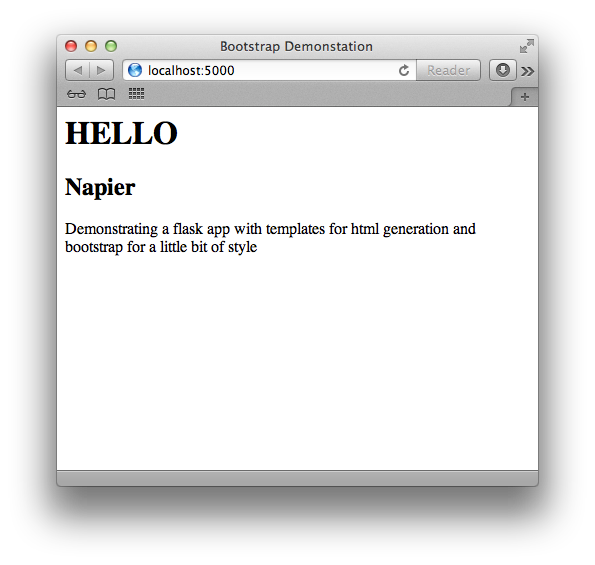
\includegraphics[width=0.85\textwidth]{images/unstyled.png}
\caption{The unstyled HTML page for the Bootstrap example}
\label{fig:unstyled}
\end{figure}

Now let's use Flask to add some basic styling to that ugly old page.

\begin{lstlisting}
<html>
<head>
  <title>Bootstrap Demonstation</title>
  <link href="{{ url_for('static', filename='css/bootstrap.min.css') }}" rel="st
</head>
<body>
<h1>HELLO</h1>
<h2>Napier</h2>
<p>Demonstrating a flask app with templates for html generation and bootstrap
for a little bit of style</p>
</body>
</html>
\end{lstlisting}

\paragraph{} Notice how all we ahve done is add a relative link, in line 4, to the Bootstrap CSS file. Also note that we used the url\_for function to get the root of the static directory and that all of the URL aspects are enclosed in Jinja2's double curly braces.  Even, just including the bootstrap CSS has already got things looking different:

\begin{figure}[H]
\centering
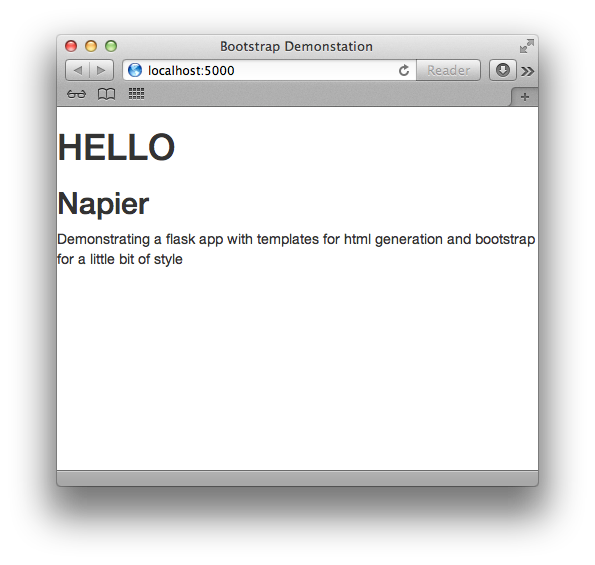
\includegraphics[width=0.85\textwidth]{images/styled-css.png}
\caption{After only including the Bootstrap CSS file}
\label{fig:styled-css}
\end{figure}

\paragraph{} But let's go a little further an implement the basic Bootstrap template:

\begin{lstlisting}
<html>
<head>
  <title>Bootstrap Demonstation</title>
  <link href="{{ url_for('static', filename='css/bootstrap.min.css') }}" rel="st
  <style>
    body{ padding-top: 50px; } <!-- Push page content down below navbar --> 
  </style>
</head>
<body>

  <nav class="navbar navbar-inverse navbar-fixed-top">
  <div class="container">
    <div class="navbar-header">
      <button type="button" class="navbar-toggle collapsed"
      data-toggle="collapse" data-target="#navbar" aria-expanded="false"
      aria-controls="navbar">
        <span class="sr-only">Toggle navigation</span>
        <span class="icon-bar"></span>
        <span class="icon-bar"></span>
        <span class="icon-bar"></span>
        </button>
        <a class="navbar-brand" href="#">ProjectName</a>
      </div>
      <div id="navbar" class="collapse navbar-collapse">
      <ul class="nav navbar-nav">
        <li class="active"><a href="#">Home</a></li>
        <li><a href="#about">About</a></li>
        <li><a href="#contact">Contact</a></li>
       </ul>
       </div>
    </div>
  </nav>
   <div class="container">
        <h1>HELLO</h1>
        <h2>Napier</h2>
        <p class="lead">Demonstrating a flask app with templates for html genera
for a little bit of style</p>
  </div>

  <script src="https://ajax.googleapis.com/ajax/libs/jquery/1.11.3/jquery.min.js
  <script src={{ url_for('static', filename='js/bootstrap.min.js') }}"></script>
</body>
</html>

\end{lstlisting}
% Add screenshot of after bootstrap



\paragraph{} The bootstrap site demonstates most of the features of bootstrap so you can see how things should look by default. It is also often useful to view the source of a given example element on the bootstrap site in order to see how it should be used.

%%%%%%%%%%%%%%%%%
%%%%%%%%%%%%%%%%%
% CHAPTER 08
%%%%%%%%%%%%%%%%%
%%%%%%%%%%%%%%%%%

\begin{comment}
\chapter{Data Storage \& Encryption}
\label{lab08}
\paragraph{} 
\end{comment}


%%%%%%%%%%%%%%%%%
%%%%%%%%%%%%%%%%%
% CHAPTER 09
%%%%%%%%%%%%%%%%%
%%%%%%%%%%%%%%%%%

\begin{comment}
\chapter{Building Data APIs with HTTP/JSON}
\label{lab09}
\paragraph{} 
\end{comment}


%%%%%%%%%%%%%%%%%
%%%%%%%%%%%%%%%%%
% CASE STUDIES 
%%%%%%%%%%%%%%%%%
%%%%%%%%%%%%%%%%%


\begin{comment}
\part{Case Studies}
\chapter{Daybook}
\label{daybook}
\paragraph{}
\end{comment}

%%%%%%%%%%%%%%%%%
%%%%%%%%%%%%%%%%%
% APPENDICES 
%%%%%%%%%%%%%%%%%
%%%%%%%%%%%%%%%%%

\appendix
\chapter{Cribsheets}
\label{cribsheets}
\paragraph{} These cribsheets are useful for collecting together lots of knew syntax but are no substitute for your own notes (and practise. Stuff you know is much better than stuff you can look up). Either way, as you learn new stuff you should expand these cribsheets with extra commands that you find useful.

\section{Linux}
\label{cribsheet_linux}

\subsection{Some useful aliases}

\begin{description}
\item[{\raise.17ex\hbox{$\scriptstyle\sim$}}] An alias that means your home directory within the filesystem hierarchy. In Levinux, for the user tc this would expand to /home/tc
\item[..] An alias that means the parent of the current directory
\end{description}

\subsection{Some useful commands}
\begin{description}
\item[cat \emph{filename}] Display the contents of the file \emph{filename}
\item[cd] Change to your home directory /home/tc or \textasciitilde/home
\item[cd \emph{..}] Change directory to the parent of the current directory
\item[cd \emph{directoryname}] Change directory to the named directory
\item[ls] List the names of the files in the current directory
\item[ls  \emph{directoryname}] List the contents of the named directory
\item[mkdir \emph{directoryname}] Create a new directory in the current directory
\item[pwd] Display the path to the current directory in the filesystem hierarchy, e.g. show you where you are relative to the root
\item[rm \emph{filename}] Delete the named file
\item[rm -rf \emph{directoryname}] Will delete the named directory and all of its contents
\item[touch \emph{filename}] Will create a new file called filename
\end{description}

\section{Vim}
\label{cribsheet_vim}
\begin{description}
\item[\$ vim] - Shell command to start a new unnamed empty document in Vim
\item[\$ vim filename.txt] - Shell command to open `filename.txt' in Vim. If it exists then the file will be opened, otherwise an empty file will be opened for editing that will be saved as `filename.txt' when you use the (w)rite command
\item[$<$ESC$>$] - Enter command Mode
\item[$<$ESC$>$i$<$ENTER$>$] Enter (i)nsert edit mode
\end{description}
\paragraph{} The following are a core set of Vim commands that are all used whilst in Command mode, e.g. after typing $<$ESC$>$
\begin{description}
\item[:q$<$ENTER$>$] - (q)uit
\item[:q!$<$ENTER$>$] - (q)uit and discard any changes
\item[:w$<$ENTER$>$] - (w)rite changes to file
\item[:wq$<$ENTER$>$] - (w)rite changes to file then (q)uit
\item[:e \emph{filename} $<$ENTER$>$] - Open file \emph{filename} in Vim for editing
\item[dd$<$ENTER$>$] - Delete the entire line that the cursor is on
\item[x$<$ENTER$>$] - Delete the character that the cursor is on
\item[j] - Move the cursor up one line (NB. You can also use the `up' arrow key
\item[k] -  Move the cursor down one line (NB. You can also use the `down' arrow key
\item[l] -  Move the cursor right one character (NB. You can also use the `right' arrow key
\item[h] -  Move the cursor left one character (NB. You can also use the `left' arrow key
\item[gg] -  Go to start of file	 
\item[G] - Go to end of file
\item[\$] - Move cursor to the end of the current line
\item[0] - Move cursor to start of current line (NB. Thats a zero)
\item[$<$CTRL$>$e] - Scroll up
\item[$<$CTRL$>$y] - Scroll down	
\item[$<$CTRL$>$b] - Page Up	
\item[$<$CTRL$>$f] - Page Down
\item[/\emph{search-term}] - Search forward for `search-term' in the current file (Use `n' for (n)ext match in current direction and (N) for next match in opposite direction)
\item[?\emph{search-term}] - Search backward for `search-term' in the current file (Use `n' for (n)ext match in current direction and (N) for next match in opposite direction)
\item[u] - Undo the last command
\item[.] - Repeat the last command
\end{description}

\paragraph{} Vim has many more commands and many ways in which individual commands can be composed into more complex composite commands. We've seen above a core set of essential commands, now we'll have a smattering of interesting further commands that are useful when editing and will give you a flavour of what Vim has to offer:
\begin{description}
\item[J] - Combine (``join'') next line with this one
\item[nG] - Move cursor to line n, e.g. 1G will take you to the first line of the file
\item[ma] - Mark current position
\item[d`a] - Delete everything from the marked position to here
\item[`a] -  Go back to the marked position] 
\item[:s/s1/s2] - Replace (``substitute'') (the first) s1 in this line by s2
\end{description}


\chapter{Annotated Code Examples}
\label{annotated}

\section{Python Flask `Hello Napier'}
\label{annotated_hello_napier}
\paragraph{} An annotated walk through the code from hello.py that we saw in section \ref{python-flask}.

\begin{lstlisting}
from flask import Flask 
app = Flask(__name__)

@app.route("/")
def hello():
    return "Hello Napier!"

if __name__ == "__main__":
    app.run(host='0.0.0.0')

\end{lstlisting}

\begin{description}
\item[Line 1] \emph{from flask import Flask}\\ 
Import the Flask class from the flask library. The library contains pre-written code and utilities that are useful when writing a web-app. In this case an instance of the Flask class will be our WSGI application.
\item[Line 2] \emph{app = Flask(\_\_name\_\_)}\\
Create an instance of the Flask class. The argument `\_\_name\_\_' is the name of the flask applications module. This is used to help flask to find resources relative to the Python module such as static web resources like image files, templates, or CSS. We also create a variable, `app', that references the newly instantiated Flask class so that we can use it later.
\item[Line 4] \emph{@app.route("/")}\\
Lines that start with @ in Python are decorators. In this case we use the route() decorator to tell Flask which URL should trigger the function that route() decorates, e.g. when a browser hits the root of the url, `/' then the hello() function is run. We use route() decorators in flask to build up our HTTP API that a browser can retrieve.
\item[Line 5] \emph{def hello():}\\
This defines a function called `hello()'. hello() is executed whenever someone requests the root url.
\item[Line 6] \emph{return "Hello Napier!"}\\
All our hello() does is to return the string ``Hello Napier''. It is this string that is displayed in the browser. We could instead return some HTML for a richer experience but plain textis sufficient for now.
\item[Line 8] \emph{if \_\_name\_\_ == "\_\_main\_\_":}\\
This is used to control how the Python module and the flask app server is run. We only want to use app.run() if this script is executed from the Python interpreter, e.g. by calling \$python hello.py. If we were to use an app server instead then the app.run() would be performed differently.
\item[Line 9] \emph{app.run(host='0.0.0.0')
}\\
Calls the run() function of the Flask app class instance to start our development server running using this app as the web app. This line also tells the app to run on a network interface that is accessible from an external address, e.g. from the Windows machine that is running Levinux, otherwise our app would only be accessible within Levinux and we don't have a graphical browser installed there.
\end{description}

\chapter{Additional Miscellaneous (but useful) Tools}
\label{additional-tools}

\section{cURL}
\label{curl}
\paragraph{} The cURL tool is a command that you can use to interact with remote HTTP APIs. It can function purely as a download tool in the terminal, for example, in Section \ref{static} we used cURL to retrieve an image file for use in our Flask static file demonstration, e.g.

\begin{lstlisting}[style=DOS]
    $ curl -L siwells.github.io/assets/images/vmask.jpg -o vmask.jpg
\end{lstlisting}

\paragraph{} By default cURL will perform an HTTP GET to the URL that we provide, However we can also specify the HTTP verb that we want to use as an additional arguments to the tool, e.g.

\begin{lstlisting}[style=DOS]
    $ curl -X POST -d "firstName=jebediah" http://dummy.com/persons/person 
\end{lstlisting}
\paragraph{} Notice the use of `-X POST' to specify the verb (which could be any verb defined by the HTTP standard, e.g. GET, POST, PUT, DELETE, HEAD, OPTIONS, \&c.). Some verbs also expect a payload so we have also included one using the `-d' argument and providing a key and value. This could actually be a whole JSON document or separate file that is used as the payload but for now we'll keep things simple.

\paragraph{} We can cause cURL to print extra information by using `-i' option and can also use `-H' to specificy the accept header for the request. In the following case indicating that the payload is of type `application/json'
\begin{lstlisting}[style=DOS]
    $ curl -i -H "Accept: application/json" -X POST -d "firstName=jebediah" http://dummy.com/persons/person 
\end{lstlisting}


\paragraph{} 

\backmatter

\bibliographystyle{plain}

\bibliography{adv-web-tech}

\end{document}

